% The FYP template is designed according to NTU SCSE FYP guidelines on https://www3.ntu.edu.sg/scse/fyp/UsefulInfo/Report%20Guide.pdf.

\documentclass[pdftex,12pt]{article}
\usepackage{newtxtext}
\usepackage[top=3cm, bottom=3cm, left=3.5cm, right=3cm]{geometry}
\usepackage[hidelinks]{hyperref}
\usepackage[pdftex]{graphicx}
% \usepackage{booktabs}
\usepackage{setspace}
\usepackage{titlesec}
% \usepackage{tocloft}
% \usepackage{parskip}
% \usepackage{amsmath}
% \usepackage{amsfonts}
% \usepackage[sorting=none]{biblatex}

%Italian-specific commands
%--------------------------------------
\usepackage[italian]{babel}
%Hyphenation rules
%--------------------------------------
\usepackage{hyphenat}
\hyphenation{mate-mati-ca recu-perare}


% change the following
\title{\uppercase{WebComics}}
\author{Alessandro Canossa - Matricola: 128434}
\date{2022}
% \newcommand\degree{}

\begin{document}
\makeatletter
\begin{titlepage}
  \begin{center}

    \uppercase{\textbf{\large{}}}
    \\[7cm]

    \textbf{\huge{\@title}}
    \\Web app per pubblicare e leggere comics

    \vfill
    \@author
    \\[3cm]

    \@date

  \end{center}
\end{titlepage}
\makeatother

\setcounter{page}{1}
\pagenumbering{roman}

\tableofcontents

\cleardoublepage
\pagenumbering{arabic}


\section{Requisiti}

Il progetto ha lo scopo di realizzare una web app per la pubblicazione di comics da parte di qualsiasi utente, 
e permetterne la lettura agli altri utenti a fronte di un pagamento con una moneta virtuale (coins).
\\Di conseguenza i requisiti dell’applicazione sono:

\subsection{Utenti}
\begin{itemize}
    \item \textbf{Anonimo:} Può visualizzare i comics presenti ed effettuare ricerche di vari comics. Può creare un account registrandosi.
    \item \textbf{Utente:} Può comprare \textit{coins} e acquistare i capitoli dei comics che vuole leggere. 
    Relativamente ai comics può dare un voto da 1 a 10 e salvarlo nella libreria. 
    Relativamente ai capitoli: può acquistarli, leggerli, mettere like, commentare e rispondere ai commenti. 
    Infine può fare richiesta di diventare Creatore.
    \item \textbf{Creatore:} può creare nuovi comic e caricare i relativi capitoli. Da una pagina apposta può controllare le informazioni dei propri comics, come voto, salvataggi in libreria e visite totali. Infine può aggiornare lo stato dei comics.
\end{itemize}


\subsection{Funzionalità}
\begin{itemize}
    \item \textbf{Creazione di comics:}
          \\Durante la creazione di un comics bisogna fornire:
          \begin{itemize}
              \item Immagine di copertina
              \item Titolo
              \item Genere (1 o più)
              \item Sinossi
          \end{itemize}
    \item \textbf{Aggiunta di un capitolo:}
          \\Una volta scelto il comic per cui aggiungere il capitolo, bisogna fornire:
          \begin{itemize}
              \item Numero del capitolo
              \item Immagini del capitolo (1 o più), con i titoli ordinati in senso di lettura.
          \end{itemize}

    \item \textbf{Commenti:}
          \\Un utente può scrivere commenti sotto i vari capitoli, eliminarli, oppure rispondere a commenti di altri utenti.
          Nel profilo personale è visualizzabile l’elenco di tutti i commenti di un utente.
    \item \textbf{Libreria:}
          \\Un utente può aggiungere un comic alla propria libreria, rimuoverlo e visualizzare l’intera libreria.
    \item \textbf{Cronologia di lettura:}
          \\Un utente può visualizzare e modificare la propria cronologia di lettura.
    \item \textbf{Rating di un comic:}
          \\ Un utente può assegnare un voto da 1 a 10 ad un comic. Il voto può anche essere modificato oppure rimosso.
    \item \textbf{Like ai capitoli:}
          \\Un utente che ha comprato tale capito può aggiungere o togliere un like ai capitoli che ha comprato.

    \item \textbf{Coins:}
          \\Nella pagina del market un utente può comprare una quantità di coins a sua scelta.
    \item \textbf{Registrazione e login:}
          \\Chiunque può creare un profilo fornendo: username, nome, cognome, email e password.
    \item \textbf{Diventare creatori:}
          \\Qualunque utente può diventare creatore mediante un pulsante nelle impostazioni del suo profilo.
    \item \textbf{Visualizzazione comic:}
          \\Nella homepage vengono mostrati i comics di cui sono stati aggiunti capitoli recentemente. Nella sezione “serie” è possibile filtrare i comics in questi modi:
          \begin{itemize}
              \item Selezionando uno o più generi di comic
              \item Selezionando uno o più stati di pubblicazione
              \item Per nome, tramite barra di ricerca
          \end{itemize}
          Inoltre i risultati possono essere ordinati per:
          \begin{itemize}
              \item Rating
              \item In ordine alfabetico
              \item Numero di aggiunte in libreria
          \end{itemize}


\end{itemize}
\break

\section{Descrizione del progetto}

\subsection{Tipologie di utenti}

\begin{itemize}
  \item \textbf{Admin:} ha la capacità di accedere al pannello amministrativo e creare,
        modificare o eliminare tutti i tipi di oggetti all’interno del database,
        può inoltre effettuare ricerche sulle entries del database e filtrare i risultati.

        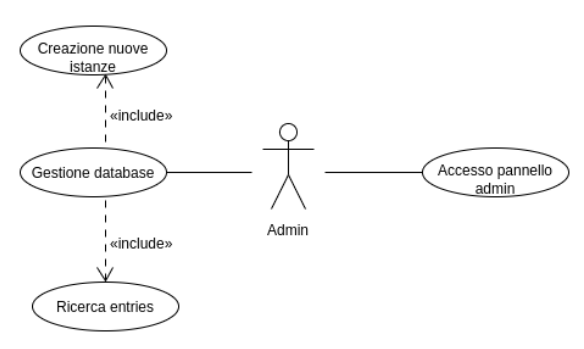
\includegraphics[width=1\linewidth]{images/admin.png}

  \item \textbf{Anonimo:} un utente non registrato ha la possibilità di effettuare ricerche
        e vedere tutti i comics disponibili. Può vedere la pagina dettagliata di un comic, ma non può accedere ai vari capitoli.
        Infine può creare un account.

        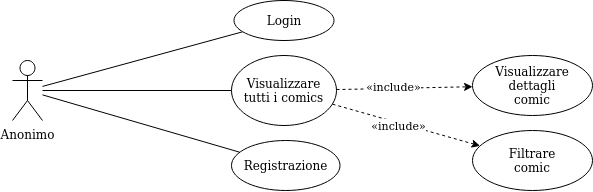
\includegraphics[width=1\linewidth]{images/anonimo.png}

  \item \textbf{Utente:} un utente registrato mantiene tutte le capacità di un utente anonimo.
        \\ L'utente può assegnare un voto da 1 a 10 ad un comic, modificare il suo voto oppure rimuoverlo.
        Può anche salvare il comic nella propria libreria.
        \\In più ha la possibilità di acquistare \textit{coins} che sono una moneta che può essere utilizzata per acquistare
        i vari capitoli di un comic.
        \\ Una volta acquistato un capitolo, l'utente può leggerlo e mettere un \textit{like},
        può lasciare commenti sotto di esso e anche rispondere ad altri commenti.
        \\ Nella pagina riservata all'utente, questo può controllare i propri commenti, i capitoli acquistati,
        i commenti lasciati, i capitoli letti e la propria libreria.
        \\Infine può modificare i propri dati personali, e può anche diventare \textbf{Creator} facendo richiesta.


        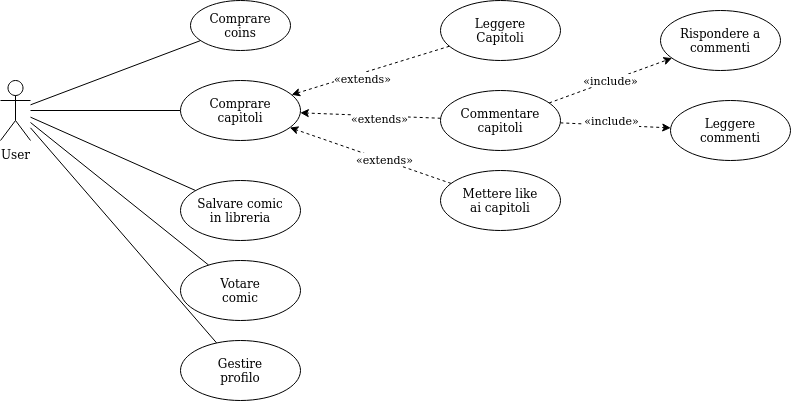
\includegraphics[width=1\linewidth]{images/utente.png}

  \item \textbf{Creator:} un utente con questo ruolo ha la possibilità di creare nuovi comics e caricarne i relativi capitoli.
        \\ Dalla propria pagina utente, può vedere i comics creati e le varie statistiche relative ai vari comics.

        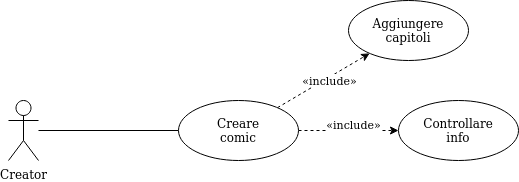
\includegraphics[width=1\linewidth]{images/creatore.png}

\end{itemize}


\subsection{Database e modelli}
Il database utilizzato per lo sviluppo del progetto è stato \textbf{Sqlite}, scelto per la
sua leggerezza e facilità di utilizzo. Nulla impedisce però di potersi spostare ad
altri database in caso di nuovi futuri requisiti.
\\I modelli (tabelle) utilizzati all’interno del database sono stati:

\subsubsection{User}
Modello usato per gestire le tipologie di utenti che possono utilizzare il sito. Per
la realizzazione è stato esteso il modello AbstractUser, presente nell’insieme di
classi messe a disposizione dal framework Django, in modo da avere già diversi
campi disponibili per l’uso.

\begin{center}
  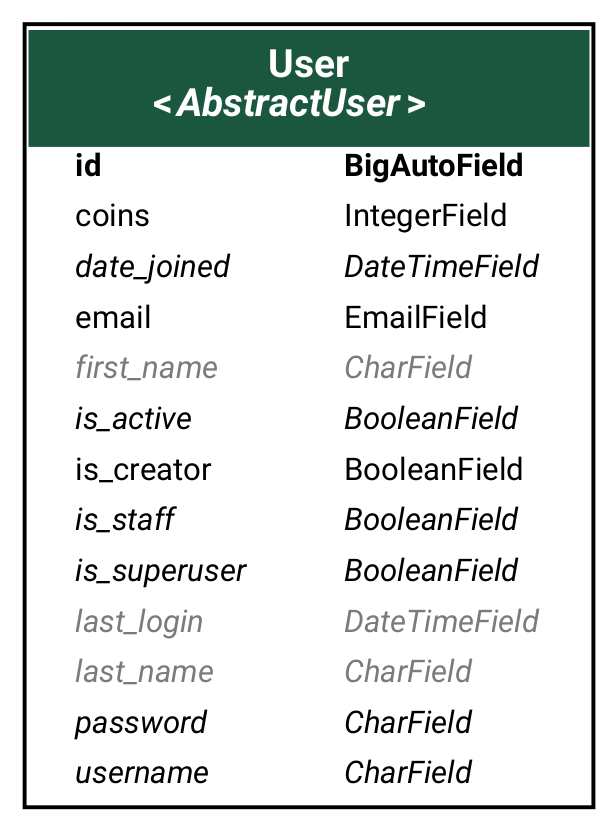
\includegraphics[width=0.4\linewidth]{images/user.png}
\end{center}

\subsubsection{CoinsPurchase}
Modello usato per registrare le transazioni di acquisto di monete di un utente.
Ha utente come chiave esterna per identificare l’utente che ha effettuato la transazione.
\begin{center}
  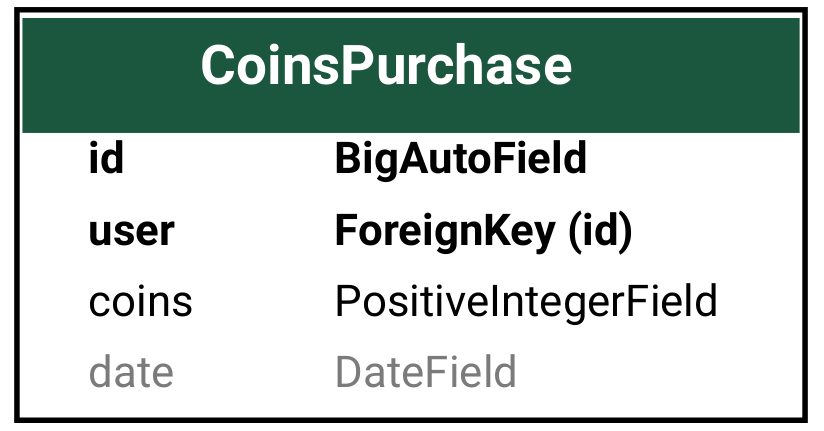
\includegraphics[width=0.4\linewidth]{images/coins-purchase.png}
\end{center}


\subsubsection{Genre}
Modello usato per gestire i generi dei comics.
\\È stato scelto di utilizzate una tabella a se stante in vista di eventuali inserimenti di nuovi generi.

\begin{center}
  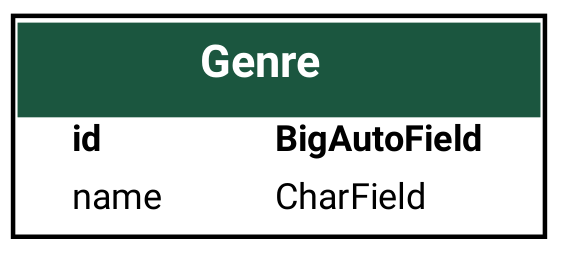
\includegraphics[width=0.4\linewidth]{images/genre.png}
\end{center}


\subsubsection{Comic}
Modello usato per gestire i dati di uno specifico comic.
Ha utente come chiave esterna per identificare l’utente che ha caricato il comic.
I campi follows, rating e watches vengono aggiornati in automatico.
Le immgini delle cover vengono salvate in una cartella che viene creata in
caso non esista.
\\La tabella \textbf{Comic} ha una relazione Many-to-Many con la tabella \textbf{Genre}, siccome un comic può avere più generi.

\begin{center}
  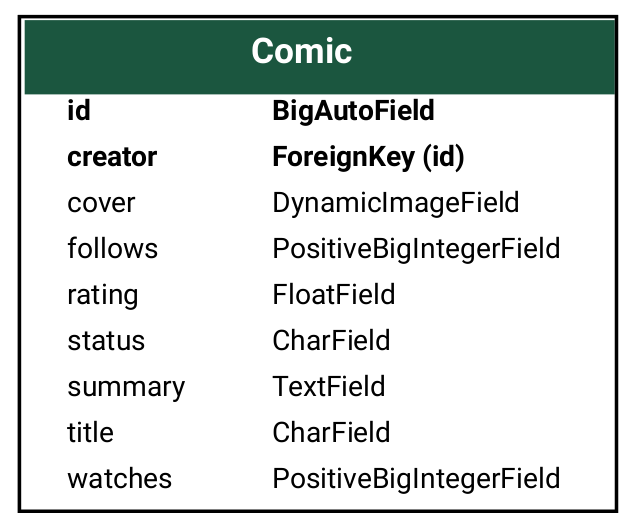
\includegraphics[width=0.4\linewidth]{images/comic.png}
\end{center}

\subsubsection{Chapter}
Modello usato per gestire i dati di un capitolo di uno specifico comic.
Anche in questo caso il campo like viene aggiornato in automatico.
\\La colonna \textbf{chapter-num} indica il numero del capitolo relativamente al comic.


\begin{center}
  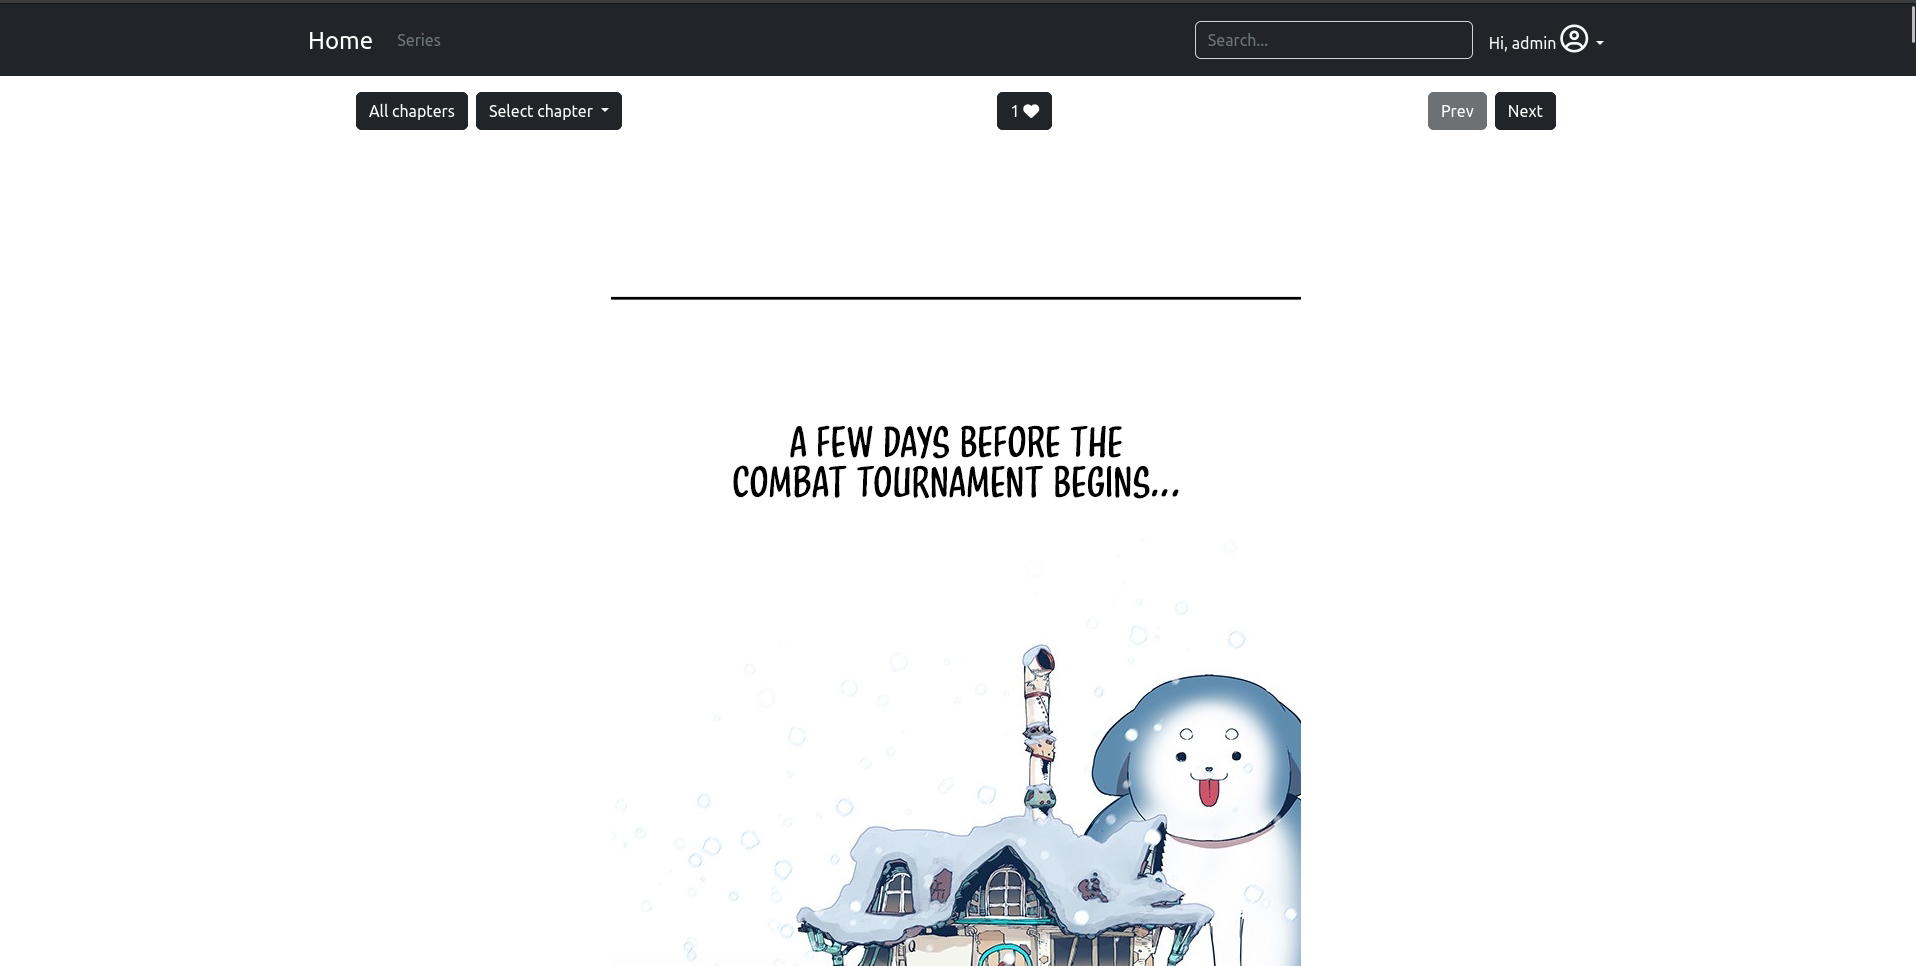
\includegraphics[width=0.4\linewidth]{images/chapter.png}
\end{center}

\subsubsection{ChapterImage}
Modello usato per gestire le immagini di un capitolo di uno specifico comic.
È stato utilizzato un modello a se stante siccomene il numero di immagini inseribili non è stato limitato.

\begin{center}
  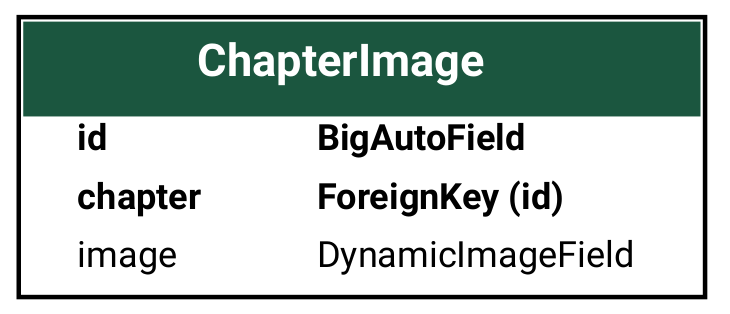
\includegraphics[width=0.4\linewidth]{images/chapter-image.png}
\end{center}

\subsubsection{BuyList}
Modello usato per gestire i capitoli acquistati da ogni utente.
Il modello è utile per consentire l'accesso ad un capitolo ai soli utenti che lo hanno acquistato.

\begin{center}
  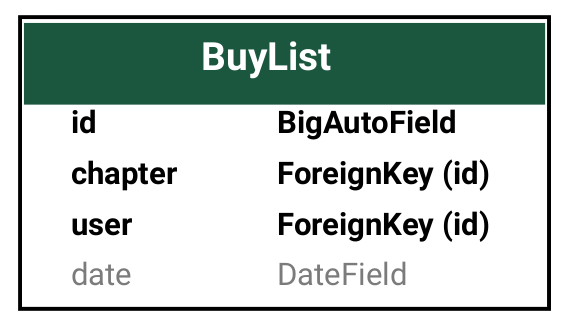
\includegraphics[width=0.4\linewidth]{images/buy-list.png}
\end{center}

\subsubsection{Rating}
Modello usato per gestire i voti di un utente ad un deteminato comic.
L'utilità del modello sta nel fatto che permette la modifica e la rimozione del voto da parte di un utente.

\begin{center}
  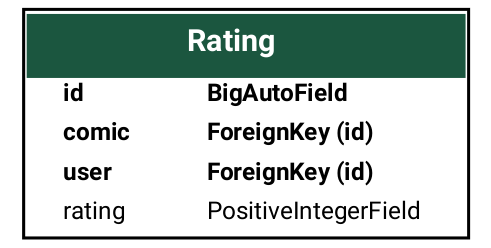
\includegraphics[width=0.4\linewidth]{images/rating.png}
\end{center}

\subsubsection{Like}
Modello usato per gestire i like di un utente ad un deteminato capitolo.
Come per il Rating, questo modello permette l'aggiunta e la rimozione di likes.

\begin{center}
  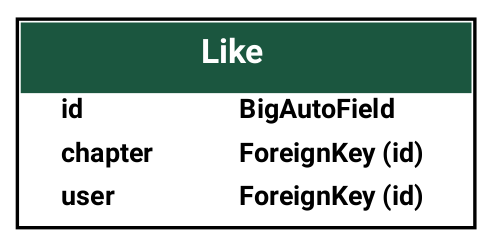
\includegraphics[width=0.4\linewidth]{images/like.png}
\end{center}

\subsubsection{Library}
Modello usato per gestire la libreria di comic di un utente.

\begin{center}
  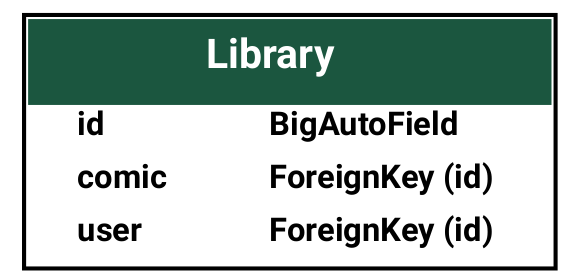
\includegraphics[width=0.4\linewidth]{images/library.png}
\end{center}

\subsubsection{ReadHistory}
Modello usato per gestire la cronologia di lettura di un utente.

\begin{center}
  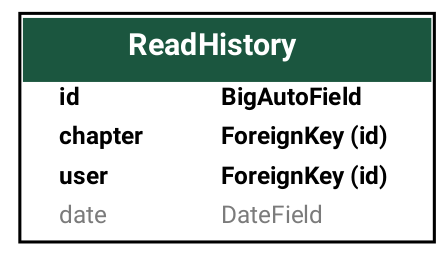
\includegraphics[width=0.4\linewidth]{images/history.png}
\end{center}

\subsubsection{Comment}
Modello usato per gestire i commenti di un utente ad un determinato capitolo.
Questo modello ha il campo \textbf{reply-to} che permette di rispondere ad altri commenti.

\begin{center}
  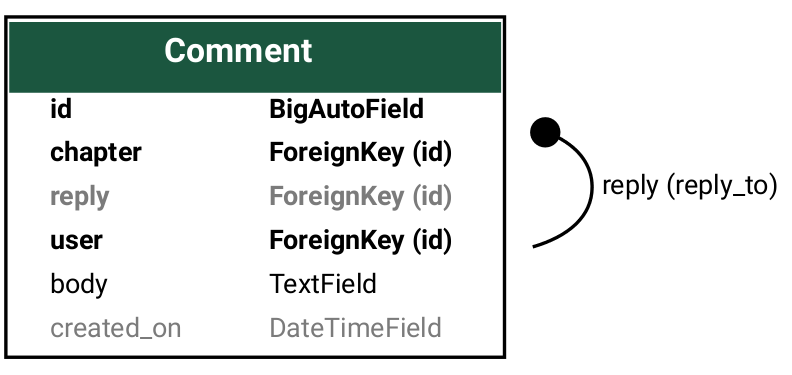
\includegraphics[width=0.4\linewidth]{images/comment.png}
\end{center}


\subsubsection{Modelli app comics}
\begin{center}
  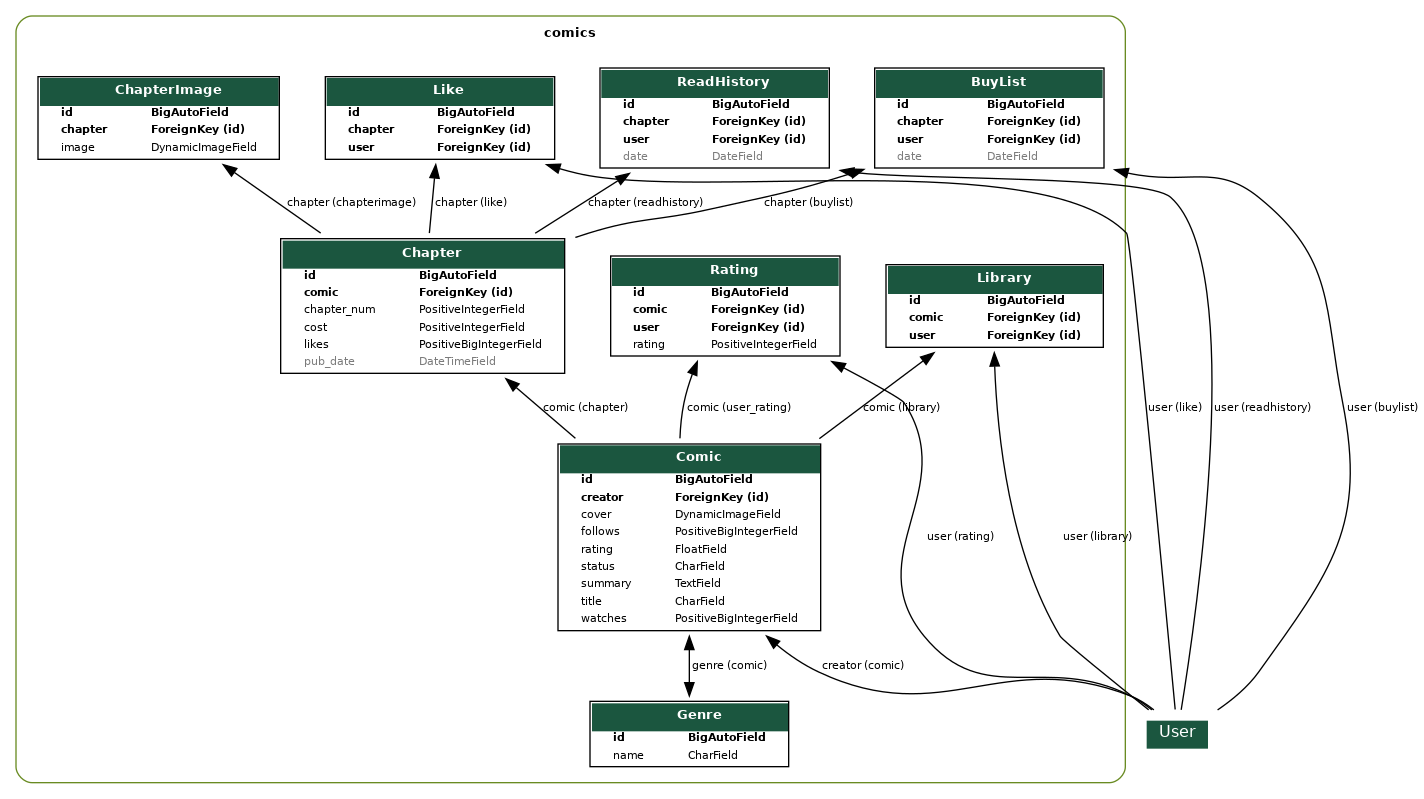
\includegraphics[width=1.0\linewidth]{images/comics.png}
\end{center}

\subsubsection{Modelli app users}
\begin{center}
  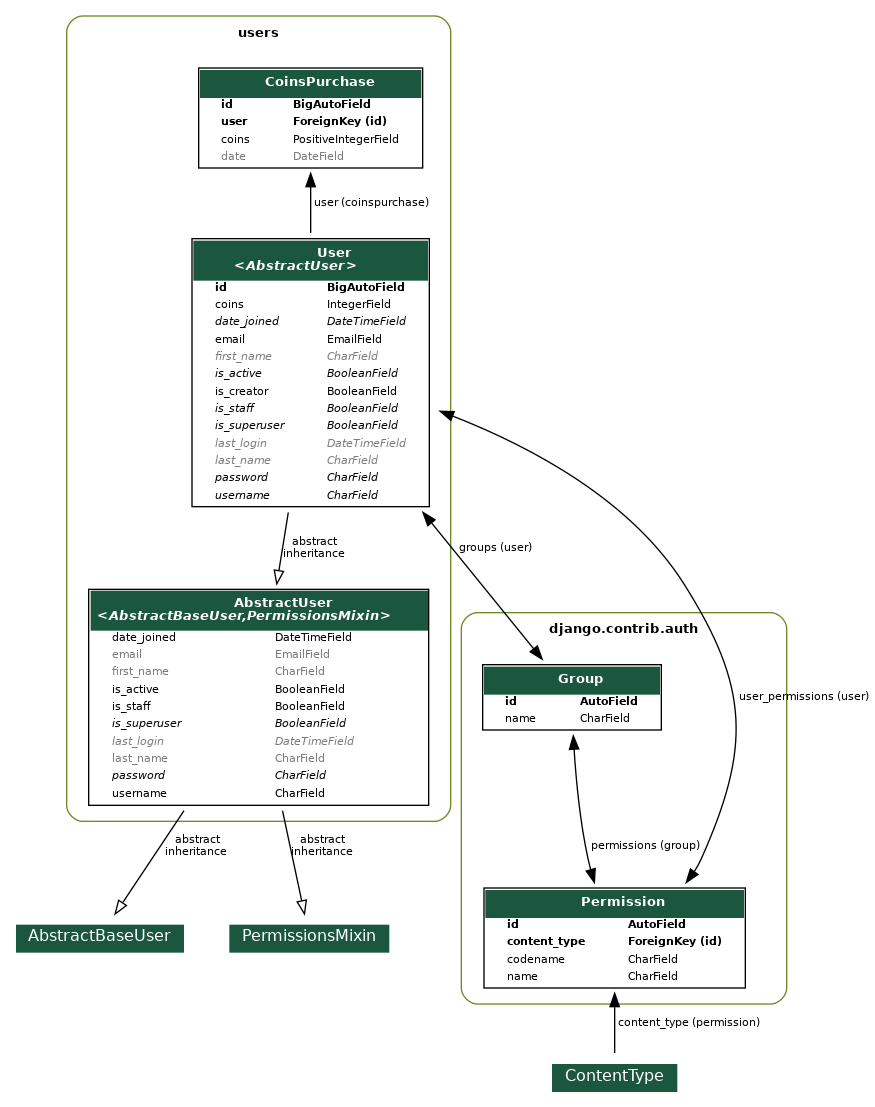
\includegraphics[width=1.0\linewidth]{images/users.png}
\end{center}

\subsubsection{Modelli app comment}
\begin{center}
  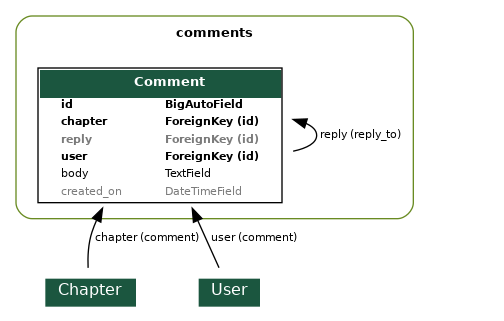
\includegraphics[width=1.0\linewidth]{images/comments.png}
\end{center}

\subsubsection{Schema completo}
\begin{center}
  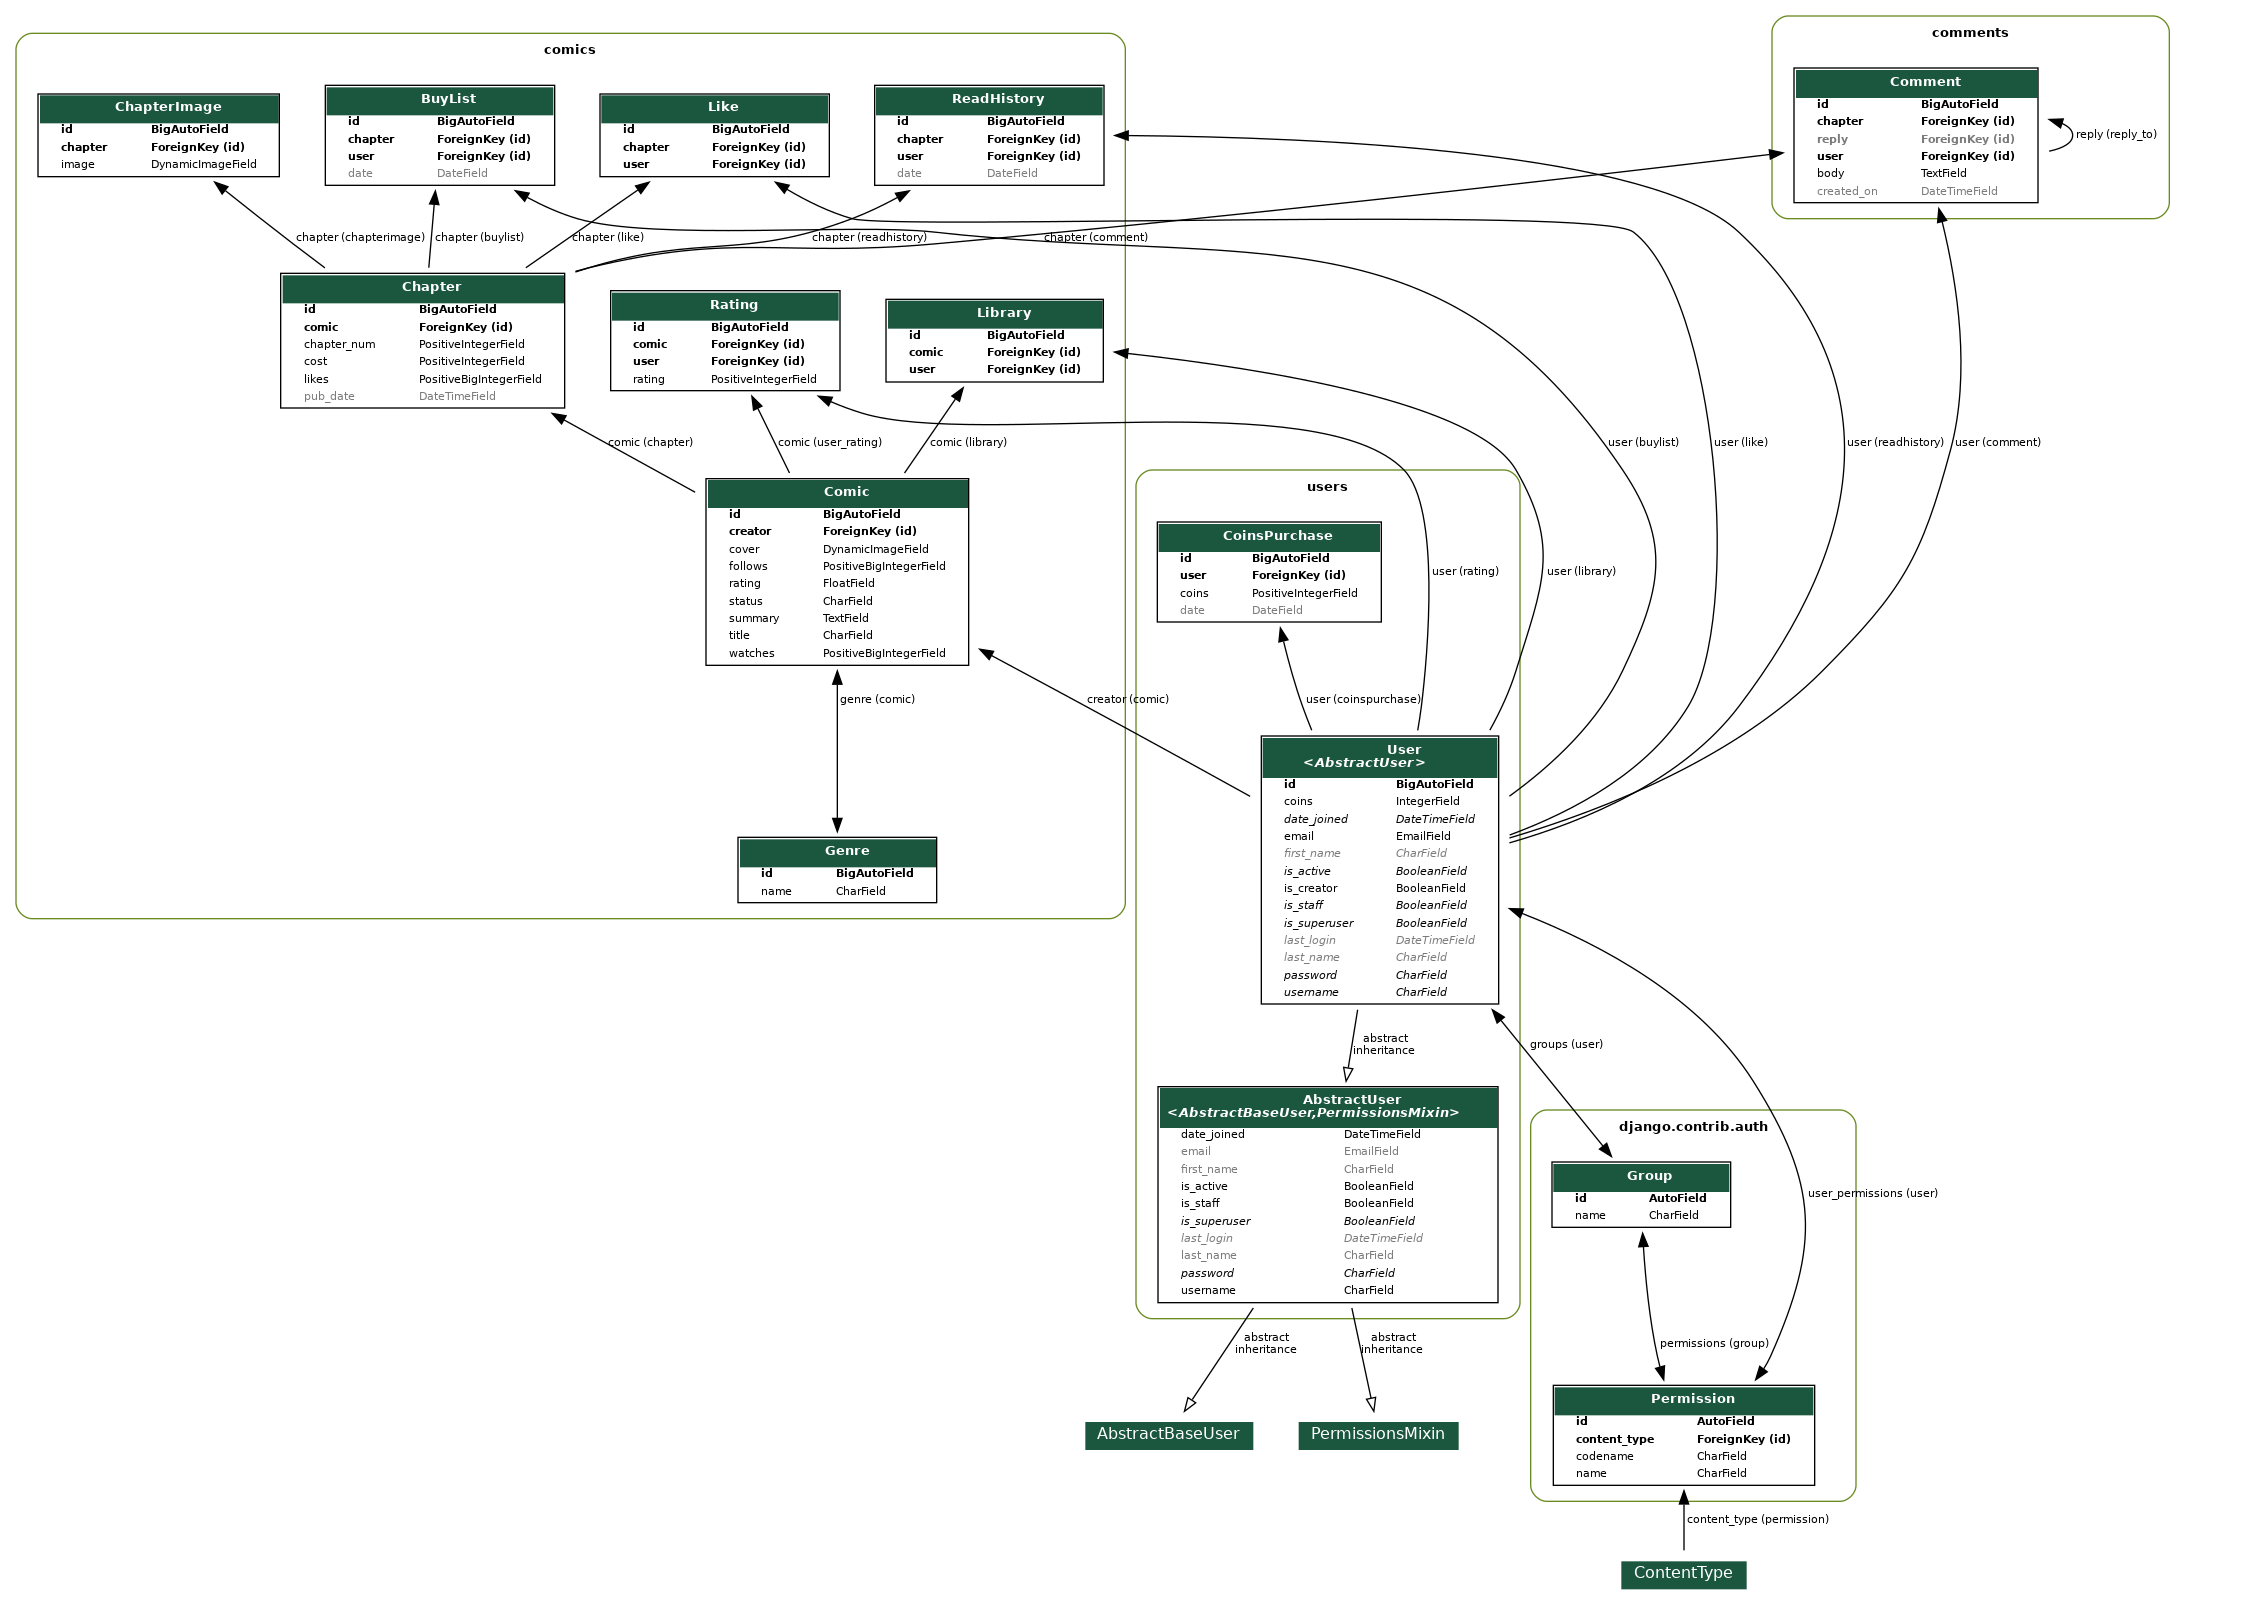
\includegraphics[width=1.3\linewidth, angle=90]{images/project.png}
\end{center}

\break

\subsection{Passaggi logici}

\begin{itemize}

  \item \textbf{Registrazione}:
        \begin{enumerate}
          \item L'utente entra nel sito.
          \item Preme il tasto \textbf{Sign up} nella navbar.
          \item Compila il form di registrazione e preme il tasto \textbf{Create account}.
        \end{enumerate}

  \item \textbf{Login}:
        \begin{enumerate}
          \item L'utente entra nel sito.
          \item Preme il tasto \textbf{Sign in} nella barra di navigazione.
          \item Compila il form di login e preme il tasto \textbf{Sign in}.
        \end{enumerate}

  \item \textbf{Logout}:
        \begin{enumerate}
          \item L'utente ha effettuato il login.
          \item Preme sull'icona utente nella barra di navigazione.
          \item Nel menù a tendina preme \textbf{Sign out}.
        \end{enumerate}

  \item \textbf{Cambio password}:
        \begin{enumerate}
          \item L'utente ha effettuato il login.
          \item Preme sull'icona utente nella barra di navigazione.
          \item Nel menù a tendina preme \textbf{User settings}.
          \item Nella barra di navigazione preme il tasto \textbf{settings}.
          \item Compila il form di cambio password e preme il tasto \textbf{Submit}.
        \end{enumerate}

  \item \textbf{Cambio username}:
        \begin{enumerate}
          \item L'utente ha effettuato il login.
          \item Preme sull'icona utente nella barra di navigazione.
          \item Nel menù a tendina preme \textbf{User settings}.
          \item Nella barra di navigazione preme il tasto \textbf{settings}.
          \item Compila il form di cambio username e preme il tasto \textbf{Submit}.
        \end{enumerate}

  \item \textbf{Comprare coins}:
        \begin{enumerate}
          \item L'utente ha effettuato il login.
          \item Preme sull'icona utente nella barra di navigazione.
          \item Nel menù a tendina preme sull'icona \textbf{coins}.
          \item Inserisce la quantità di coins da comprare e preme il tasto \textbf{Buy}.
        \end{enumerate}

  \item \textbf{Comprare un capitolo}:
        \begin{enumerate}
          \item L'utente ha effettuato il login.
          \item Preme sul comic desiderato.
          \item Nella pagina del comic, preme sul capitolo desiderato.
          \item Nel popup che appare preme il pulsante \textbf{Buy}.
        \end{enumerate}

  \item \textbf{Dare un voto a un comic}:
        \begin{enumerate}
          \item L'utente ha effettuato il login.
          \item Preme sul comic desiderato.
          \item Nella pagina del comic, preme sul tasto con una icona di una stella.
          \item Nel menù a tendina che compare preme sul voto scelto.
        \end{enumerate}

  \item \textbf{Aggiungere un comic alla libreria}:
        \begin{enumerate}
          \item L'utente ha effettuato il login.
          \item Preme sul comic desiderato.
          \item Nella pagina del comic, preme sul tasto \textbf{Bookmark}.
        \end{enumerate}

  \item \textbf{Scrivere un commento}:
        \begin{enumerate}
          \item L'utente ha effettuato il login.
          \item Preme sul comic desiderato.
          \item Nella pagina del comic, preme sul capitolo desiderato.
          \item Scorre la pagina fino alla sezione commenti.
          \item Compila il form di commento e preme il tasto \textbf{Post}.
        \end{enumerate}

  \item \textbf{Cercare un comic}:
        \begin{enumerate}
          \item Inserisce il nome del comic nella barra di ricerca.
          \item Preme il tasto \textbf{Invio} sulla tastiera.
        \end{enumerate}

  \item \textbf{Diventare Creator}:
        \begin{enumerate}
          \item L'utente ha effettuato il login.
          \item Preme sull'icona utente nella barra di navigazione.
          \item Nel menù a tendina preme \textbf{User settings}.
          \item Nella pagina utente navigare fino alla sezione \textbf{Settings}.
          \item Premere il tasto \textbf{Become Creator}.
        \end{enumerate}

  \item \textbf{Creare un nuovo comic}:
        \begin{enumerate}
          \item L'utente ha effettuato il login.
          \item Preme sull'icona utente nella barra di navigazione.
          \item Nel menù a tendina preme \textbf{user settings}.
          \item Nella pagina utente navigare fino alla sezione \textbf{My comics}.
          \item Premere il pulsante \textbf{Add new comic}.
          \item Compilare il form di creazione del comic e preme il tasto \textbf{Add comic}.
        \end{enumerate}

  \item \textbf{Creare un nuovo capitolo}:
        \begin{enumerate}
          \item L'utente ha effettuato il login.
          \item Preme sull'icona utente nella barra di navigazione.
          \item Nel menù a tendina preme \textbf{user settings}.
          \item Nella pagina utente navigare fino alla sezione \textbf{My comics}.
          \item Premere il pulsante \textbf{Add chapter} sul comic desiderato.
          \item Compilare il form di creazione del capitolo e preme il tasto \textbf{Add new chapter}.
        \end{enumerate}

\end{itemize}


\break
\section{Tecnologie usate}

\subsection{Backend}
Per il backend della web app è stato utilizzato il framework web visto a lezione, ovvero Django.
Si è scelto di adottare questo framework perché permette una grande velocità
di sviluppo una volta che si è capito il meccanismo di funzionamento. Permette
anche di astrarre tutte le complessità legate alla gestione di un database e alla
creazione dinamica dei templates delle pagine con i dati ottenuti dal database.
\\Per la maggior parte delle viste è stato utilizzato il template engine di Django.
Ogniuna di tali viste è legata ad un template e gestisce la logica di ottenimento di quello che
deve essere fatto vedere a schermo e/o la modifica di questi oggetti all’interno
del database.
\\Sono state però create anche delle viste che forniscono dei più semplici servizi,
come per esempio l'aggiunta di un voto ad un comic, le quali restitusicono solo
messaggi di successo o di errore.
\\Come database è stato utilizzato \textbf{SQLite3}, siccome è molto leggero,
l'app non necessita di funzioni di gestione del database particolari e anche perché
è il database che viene fornito di base da Django.


\subsection{Frontend}
Per la realizzazione del Frontend sono stati usati i template di Django,
che permettono di creare pagine dinamiche con i dati ottenuti dal database.
Inoltre forniscono anche la possibilità di creare componenti HTML riutilizzabili
e la possibilità di estendere pagine con altri template mediante l'utilizzo dei blocchi.
\\Come libreria grafica è stata utilizzata \textbf{Bootstrap}, per la facilità di
creazione degli oggetti.
\\Per la dinamicità delle pagine è stato usato anche \textbf{Javascript}, e in particolare
\textbf{AJAX}, per la gestione di bottoni e piccoli form, ad esempio per il tasto di voto.

\break
\section{Organizzazione del software}
Il progetto è stato diviso in tre app:

\subsection{users}
Applicazione in cui sono gestiti tutti i dettagli di un utente all’interno del sito;
qui è salvato il modello che rappresenta un utente, che estende quello base di
Django aggiungendo maggiori dettagli, e anche il modello che rappresenta gli acquisti di \textit{coins}.
Inoltre in questa applicazione sono state scritte tutte le views che permettono
la creazione e la modifica di un utente, oltre che la gestione del login, del logout e del cambio della password.

\subsection{comics}
In questa app sono presenti tutti i modelli che riguardano i Comic nella loro interezza,
come il modello \textit{Comic}, che rappresenta un singolo Comic, e il modello \textit{Chapter}
che rappresenta un singolo capitolo di un Comic, ma anche modelli come \textit{Library} che rappresenta
la libreria di Comic di un utente.
\\L'applicazione contiene anche tutta la logica per la creazione dei comic e dei capitoli,
per la ricerca con filtri dei comic, per la gestione dei voti, per la gestione dei comic in libreria,
per l'acquisto dei capitoli e la loro visualizzazione.


\subsection{comments}
Questa applicazione si occupa di gestire i soli commenti.
È stata tenuta separata dalle altre due app siccome in questo modo si ha la possibilità
di usarla in altri progetti andando a modificare solo poche cose.

\break
\section{Scelte effetuate}

\subsection{Viste}
Le viste sono state realizzate mediante funzioni, invece che classi,
per la possibilità di personalizzazione di fuzionamento,
a discapito del possibile utilizzo di mixins.
Questo ha portato a dover effettuare spesso controlli sui permessi degli utenti.

\subsection{AJAX}
L'utilizzo di AJAX è stato scelto per la possibilità di gestione dinamica
di pagine altrimenti statiche. Principalmente è stato utilizzato per bottoni
e piccoli form che non avrebbe avuto senso gestire con pagine separate.

\subsection{AUTH}
L'utilizzo di django auth è stato limitato al solo login e logout,
per evitare di andare a creare pagine superflue, come quella di conferma cambio password.
\\Per le notifiche di conferma cambio password e altre notifiche simili sono stati utilizzati
gli \textit{alert} di Javascript in combo con AJAX.

\subsection{Pannello admin}
Il pannello di gestione dell'admin è stato esteso con funzioni di ricerca e filtraggio per ogni modello presente.
Questo permette una ricerca più efficiente e una visualizzazione più compatta.

\subsection{Immagini}
La gestione delle immagini inizialmente si è rivelata abbastanza complicata,
ma grazie al pacchetto \textit{django-dynamic-image} si è potuto creare dinamicamente
i path di salvataggio delle immagini, in base a comic e numero di capitolo.

\break
\section{Test eseguiti}

Il progetto non è stato testato nella sua interezza, ma si è testato principalmente l'app users,
per verificare che le varie viste e il model manger funzionassero a dovere.

\subsection{UserManager}
\subsubsection{test\_create\_user}
Test utilizzato per controllare che il nuovo utente sia creato correttamente, con i campi popolati come voluto.

\subsubsection{test\_create\_superuser}
Test utilizzato per controllare che il nuovo super utente sia creato correttamente, con i campi popolati come voluto.


\subsection{UserModel}
\subsubsection{setUp}
Funzione che crea l'utente usato per i vari test.

\subsubsection{test\_login}
Test utilizzato per verificare che il login avvenga correttamente.

\subsubsection{test\_login\_invalid\_credentials}
Test utilizzato per verificare che il login fallisca con credenziali errate.

\subsubsection{test\_create\_existing\_user}
Test utilizzato per verificare l'impossibilità di creare un utente con credenziali di un utente già esistente.

\subsubsection{test\_create\_user\_with\_email\_invalid}
Test utilizzato per verificare l'impossibilità di creare un utente con un indirizzo email non valido.

\subsubsection{test\_create\_user\_with\_username\_invalid}
Test utilizzato per verificare l'impossibilità di creare un utente con un username non valido.

\subsubsection{test\_create\_user\_with\_email\_and\_username\_invalid}
Test utilizzato per verificare l'impossibilità di creare un utente con un indirizzo email e un username non validi.

\subsubsection{test\_create\_user\_with\_password\_invalid}
Test utilizzato per verificare l'impossibilità di creare un utente con una password non valida.

\subsection{UserViews}
\subsubsection{setUp}
Funzione che crea l'utente usato per i vari test.

\subsubsection{test\_logout}
Test utilizzato per verificare che la view di logout riporti alla home page.

\subsubsection{test\_change\_username}
Test utilizzato per verificare che la view di cambio username cambi correttamente l'username.

\subsubsection{test\_change\_username\_invalid\_username}
Test utilizzato per verificare che la view di cambio username non cambi l'username con un username non valido.

\subsubsection{test\_change\_username\_invalid\_username\_length}
Test utilizzato per verificare che la view di cambio username non cambi l'username con un username di lunghezza non valida.

\subsubsection{test\_change\_password}
Test utilizzato per verificare che la view di cambio password cambi correttamente la password.

\subsubsection{test\_change\_password\_invalid\_old\_password}
Test utilizzato per verificare che la view di cambio password non cambi la password se la password vecchia inserita è sbagliata.

\subsubsection{test\_buy\_coins}
Test utilizzato per verificare che la view di acquisto di coins aggiorni correttamente il numero di coins dell'utente.

\subsubsection{test\_buy\_coins\_invalid\_amount}
Test utilizzato per verificare che la view di acquisto di coins non aggiorni il numero di coins dell'utente se viene inserito un valore negativo.

\subsubsection{test\_buy\_coins\_invalid\_amount\_string}
Test utilizzato per verificare che la view di acquisto di coins non aggiorni il numero di coins dell'utente se viene inserito un valore non numerico.

\subsubsection{test\_buy\_coins\_invalid\_amount\_zero}
Test utilizzato per verificare che la view di acquisto di coins non aggiorni il numero di coins dell'utente se viene inserito un valore nullo.

\subsubsection{test\_buy\_coins\_not\_logged}
Test utilizzato per verificare che la view di acquisto di coins riporti alla pagina di login se l'utente non è loggato.

\subsubsection{test\_buy\_coins\_entry\_created}
Test utilizzato per verificare che la view di acquisto di coins crei una entry nella tabella delle transazioni.

\subsubsection{test\_buy\_coins\_entry\_created\_invalid\_amount}
Test utilizzato per verificare che la view di acquisto di coins non crei una entry nella tabella delle transazioni se viene inserito un valore non valido.

\subsubsection{test\_become\_creator}
Test utilizzato per verificare che la view per diventare creator cambi correttamente il campo is\_creator dell'utente se l'utente è loggato.

\subsubsection{test\_become\_creator\_not\_logged}
Test utilizzato per verificare che la view per diventare creator non cambi il campo is\_creator dell'utente se l'utente non è loggato.

\subsubsection{test\_become\_creator\_already\_creator}
Test utilizzato per verificare che la view per diventare creator non cambi il campo is\_creator dell'utente se l'utente è già creator.

\break
\section{Risultati ottenuti}

\subsection{Homepage}
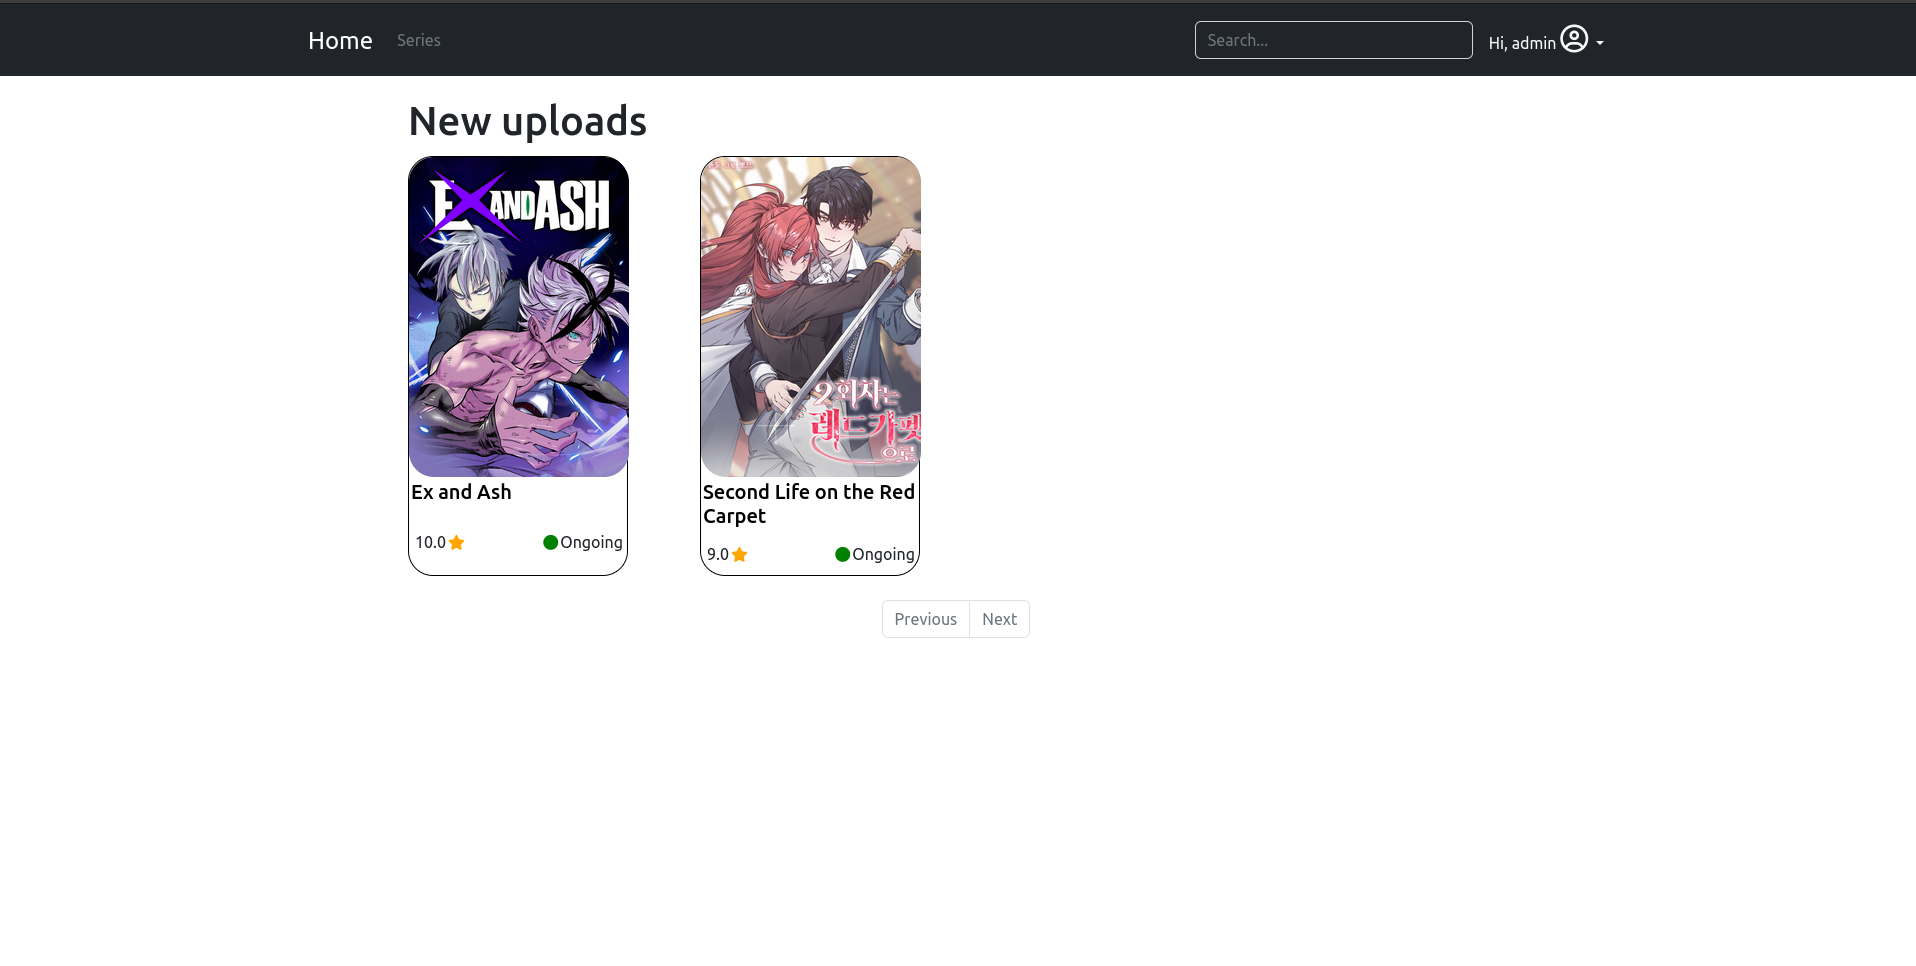
\includegraphics[width=1.0\linewidth]{images/homepage.png}

\subsection{Series}
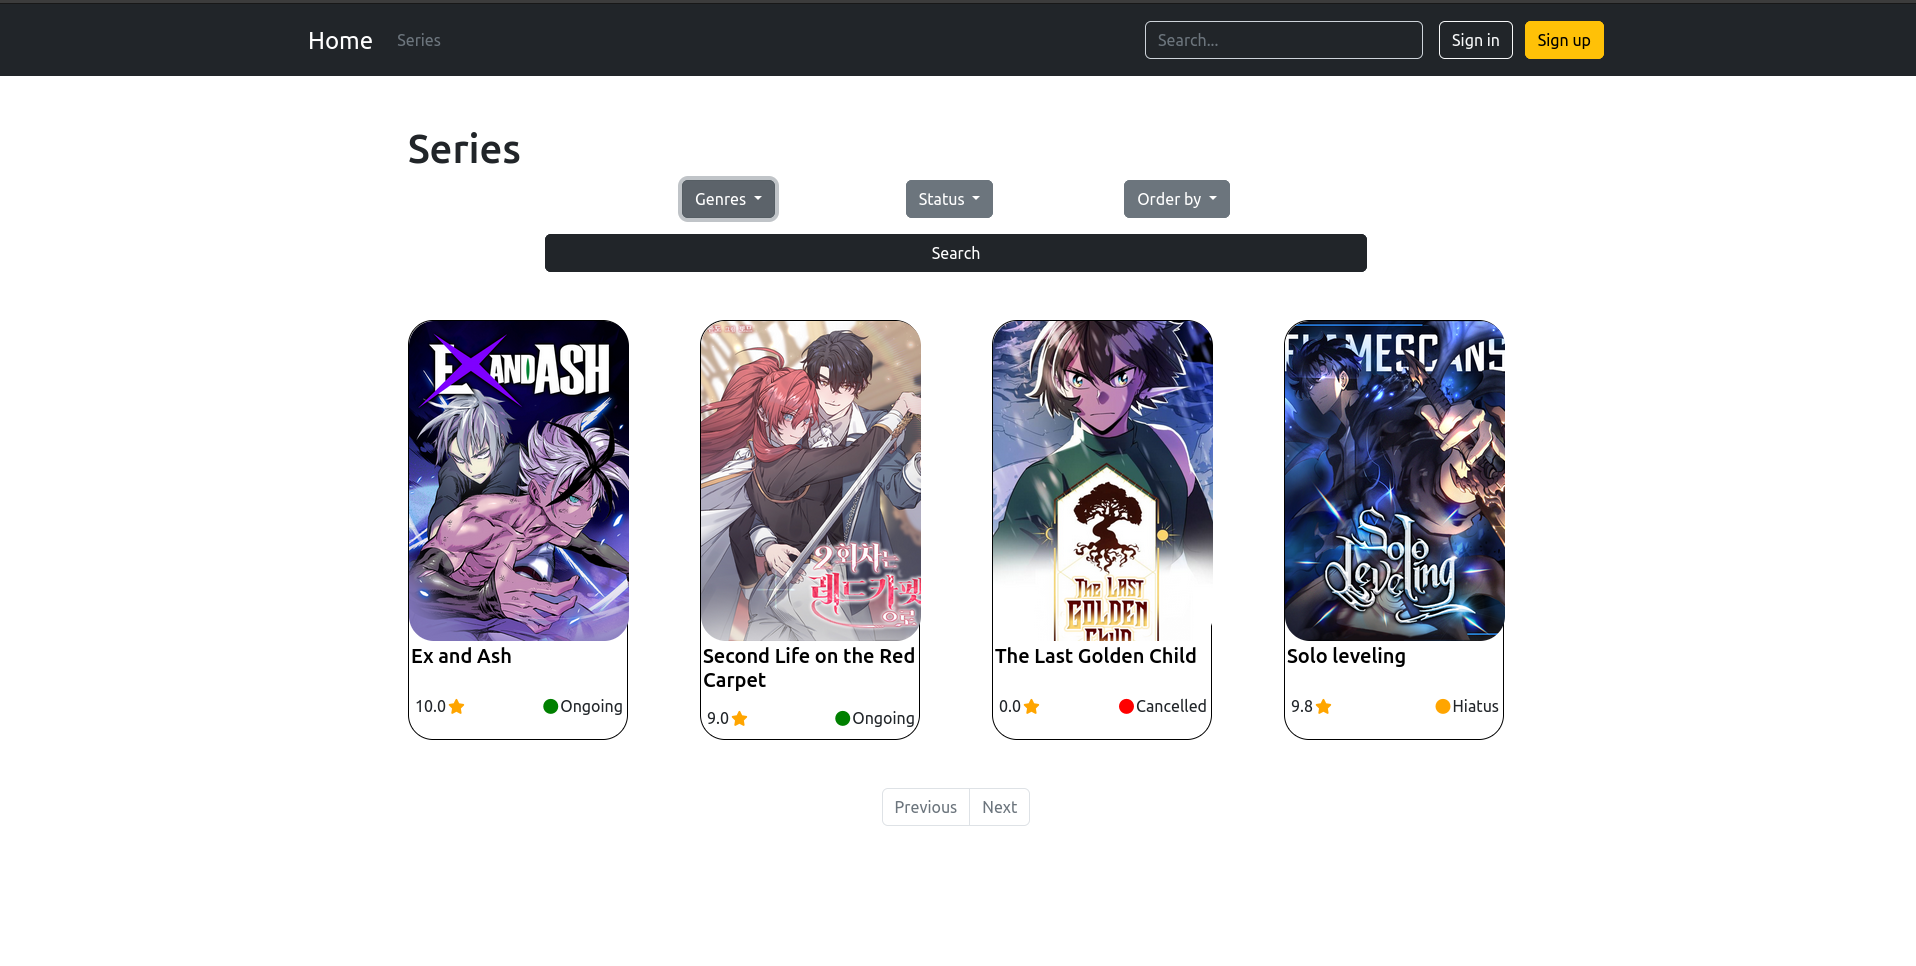
\includegraphics[width=1.0\linewidth]{images/comic-list.png}

\subsection{Comic}
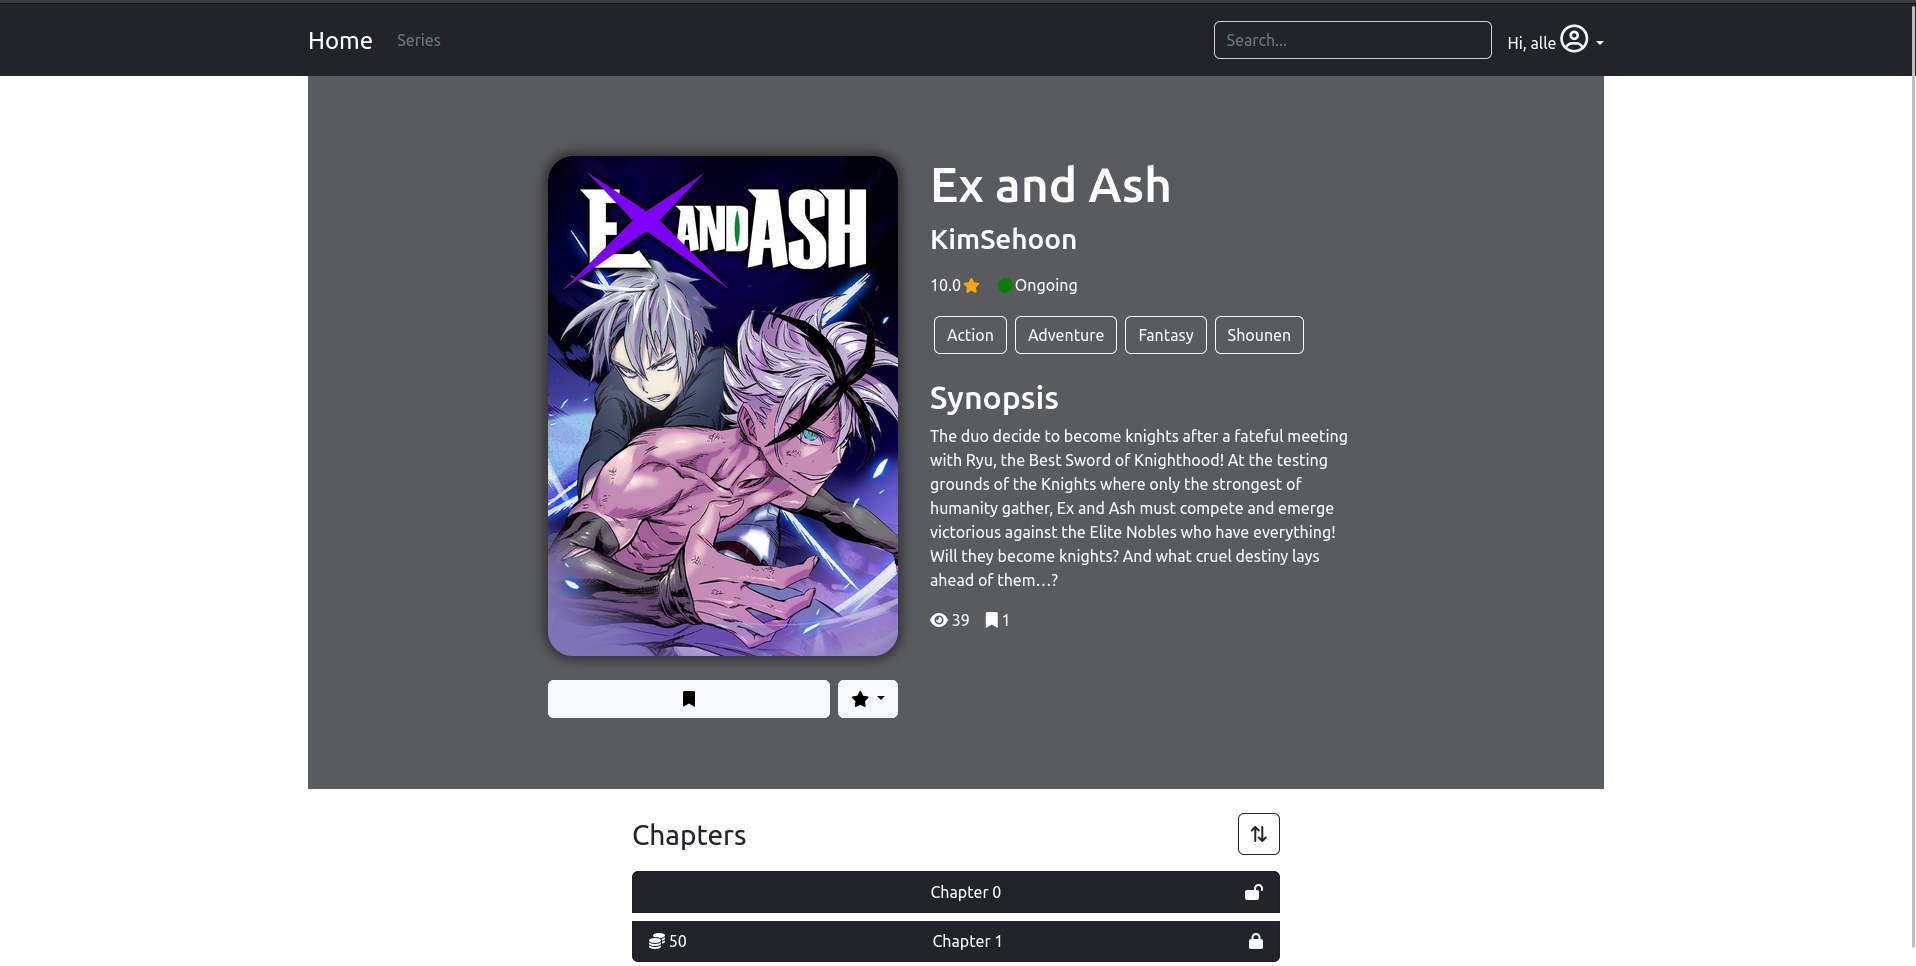
\includegraphics[width=1.0\linewidth]{images/comic-detail.png}

\subsection{Chapter}
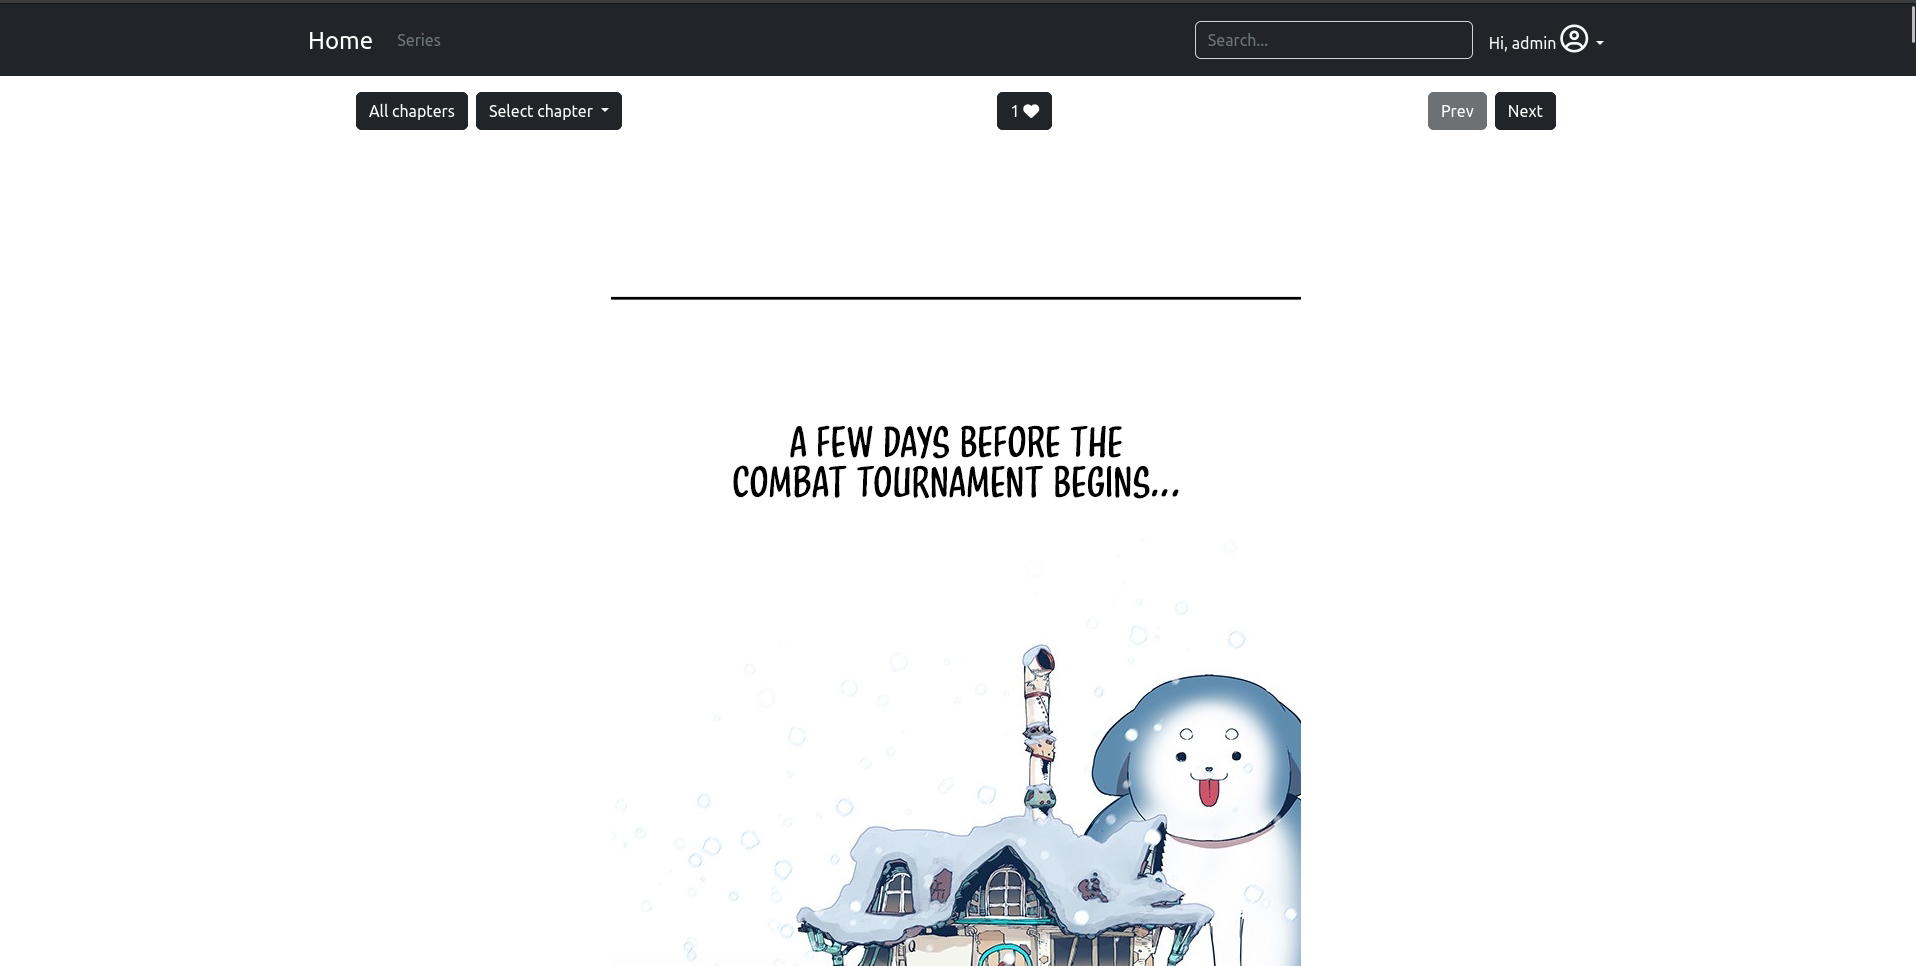
\includegraphics[width=1.0\linewidth]{images/chapter.png}

\subsection{Login}
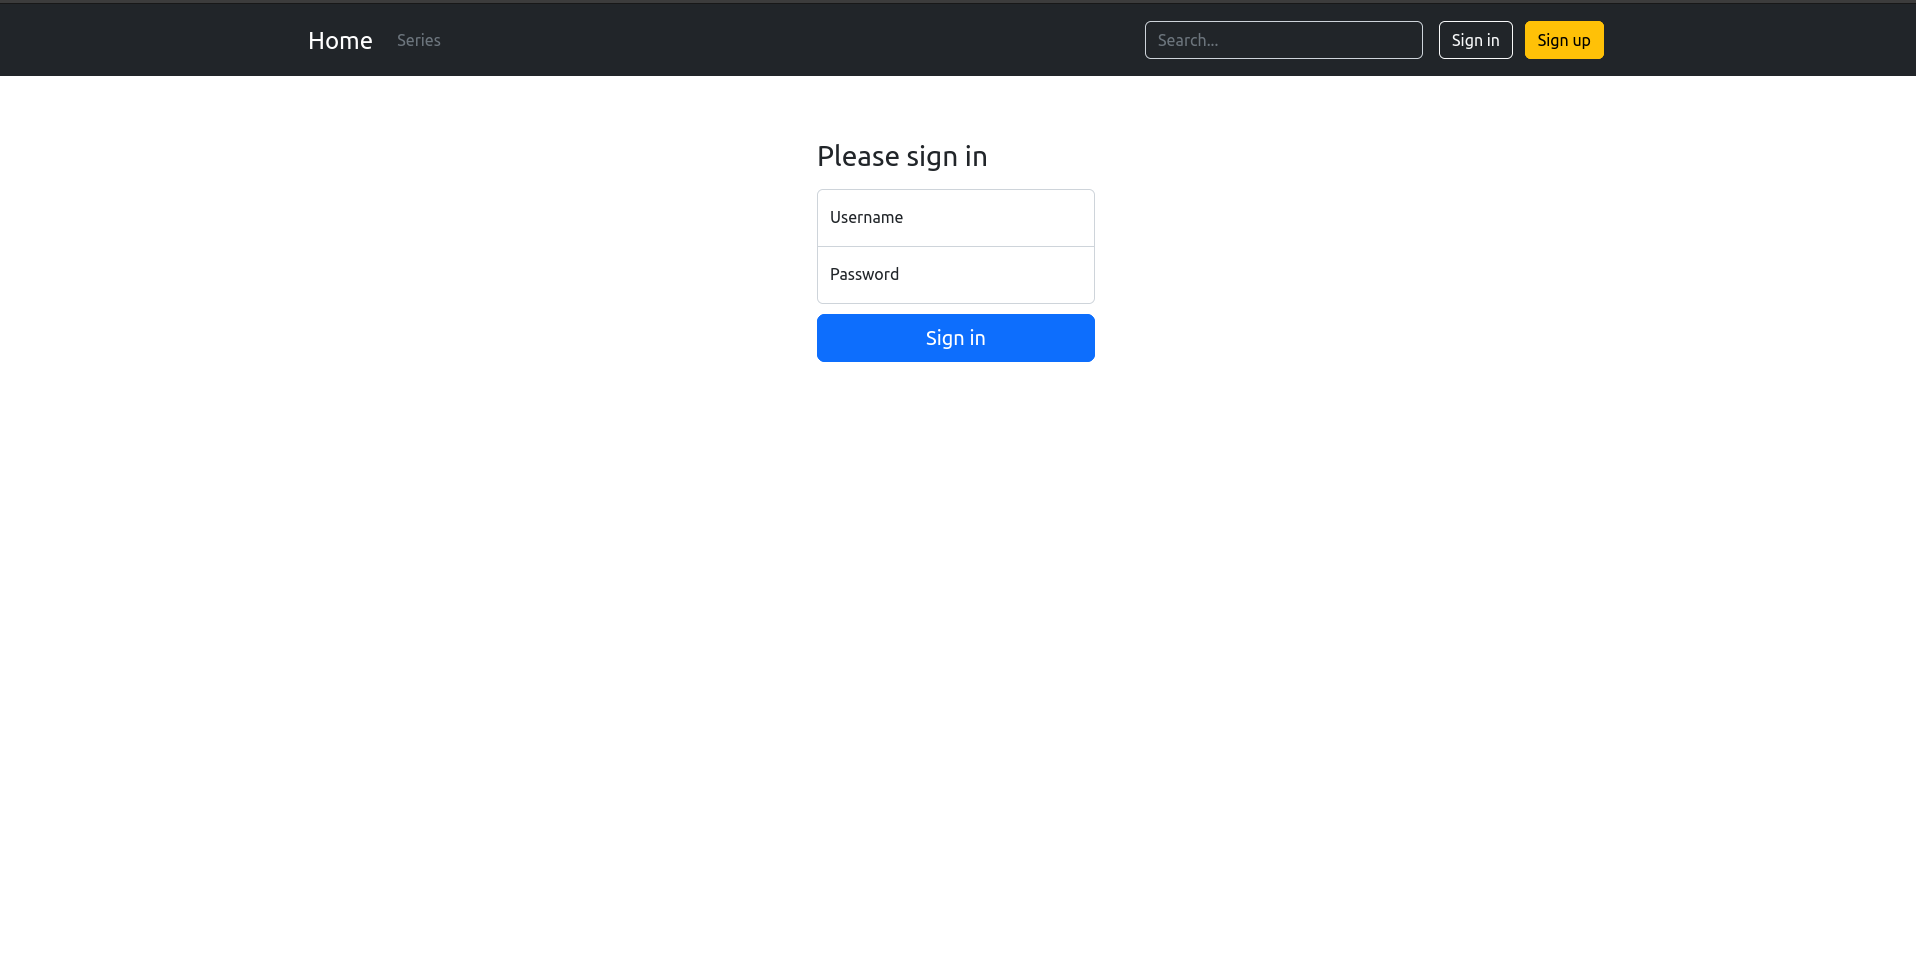
\includegraphics[width=1.0\linewidth]{images/login.png}

\subsection{Register}
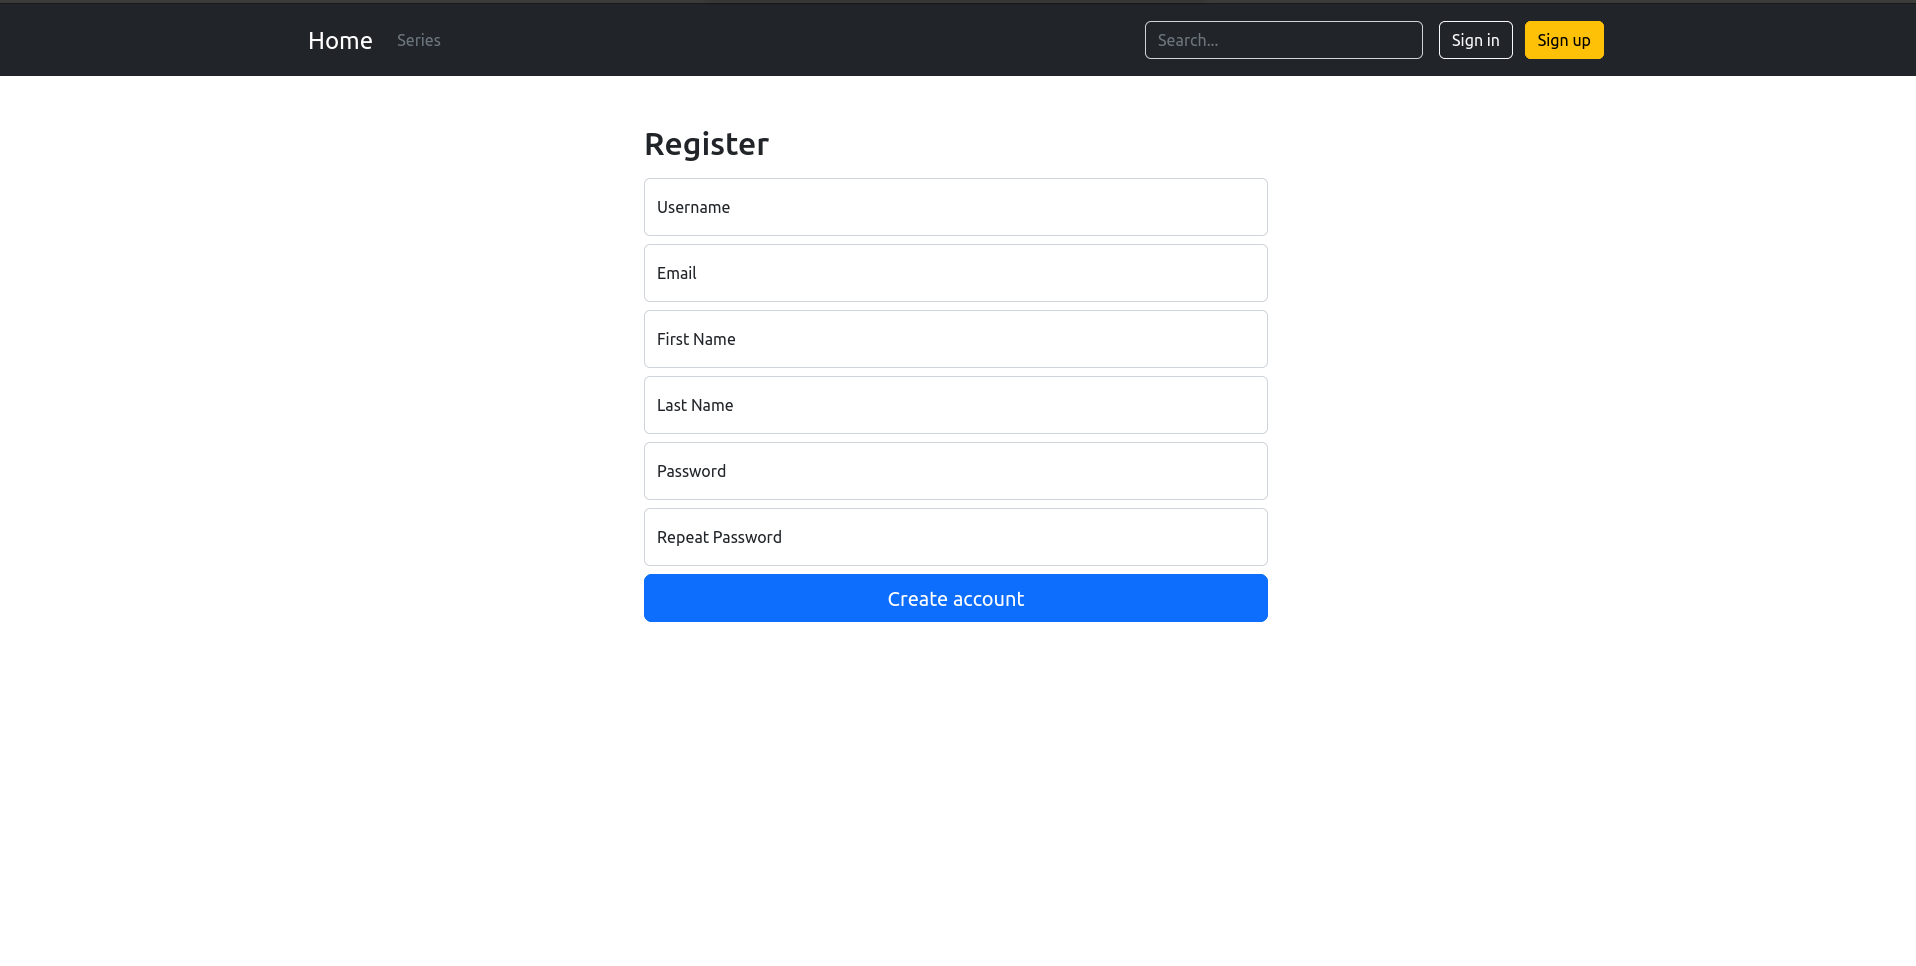
\includegraphics[width=1.0\linewidth]{images/registration.png}

\subsection{User Settings}
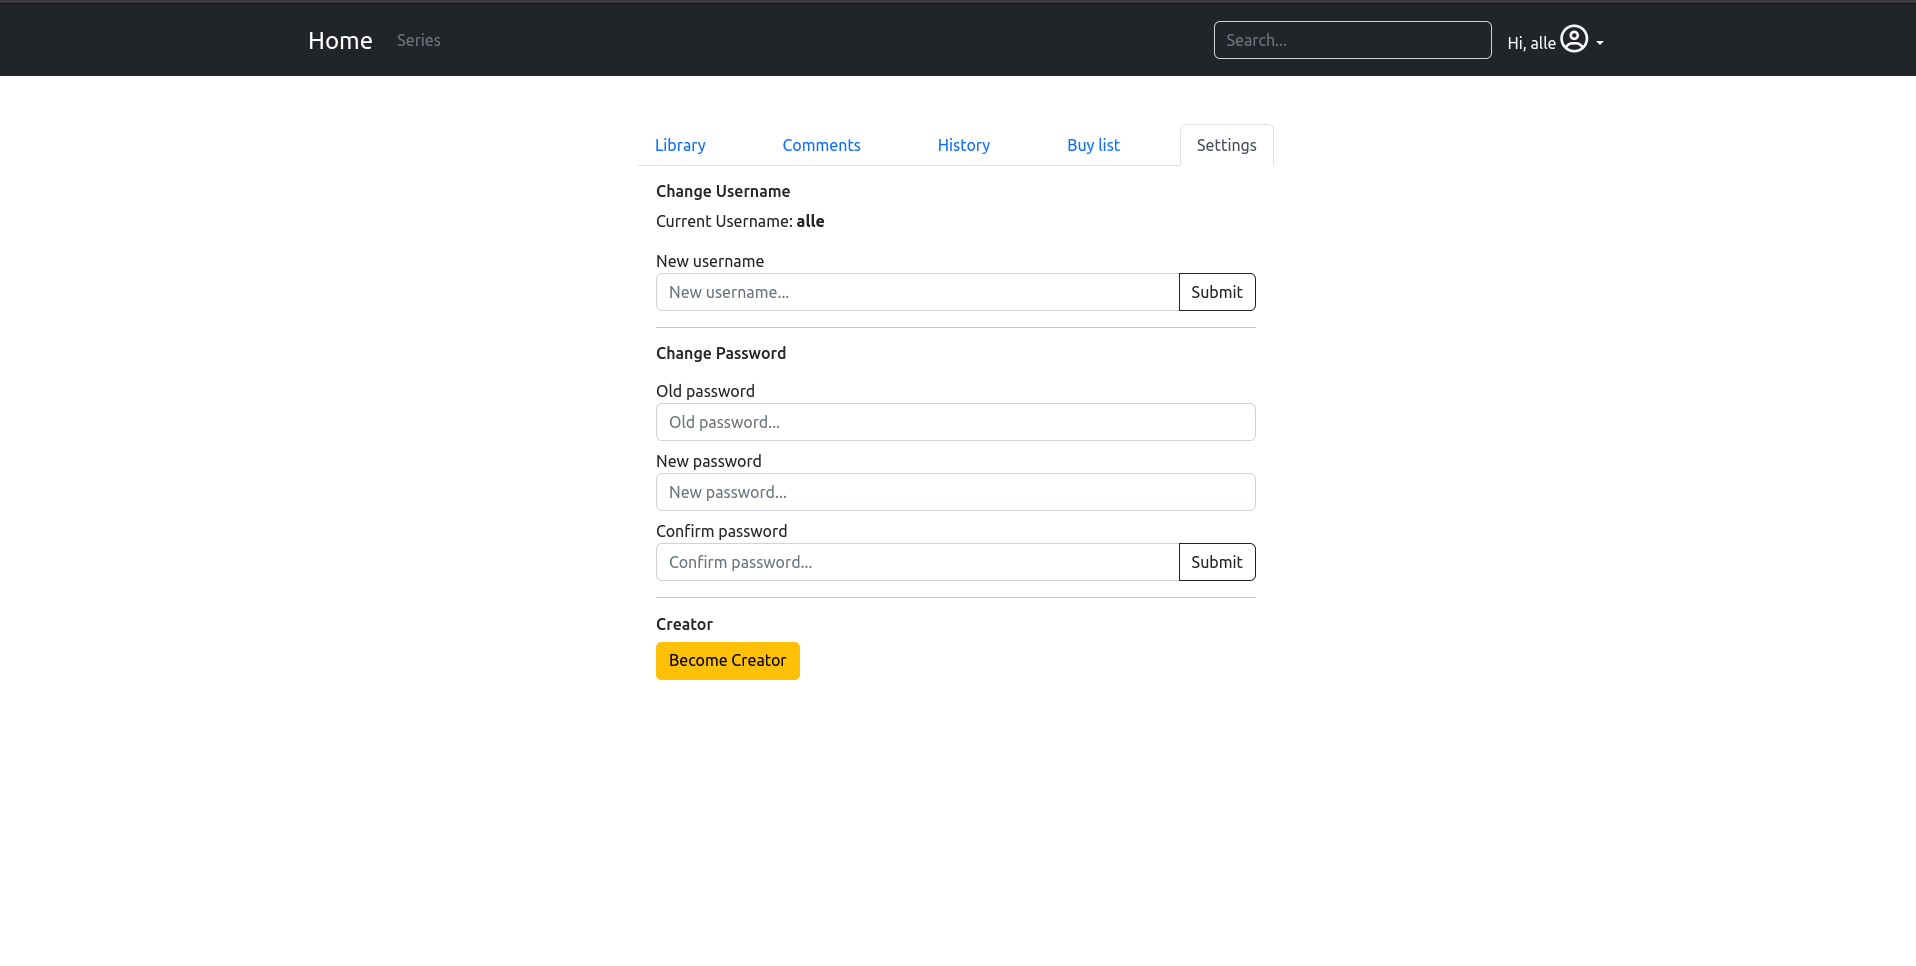
\includegraphics[width=1.0\linewidth]{images/user-settings.png}

\subsection{Market}
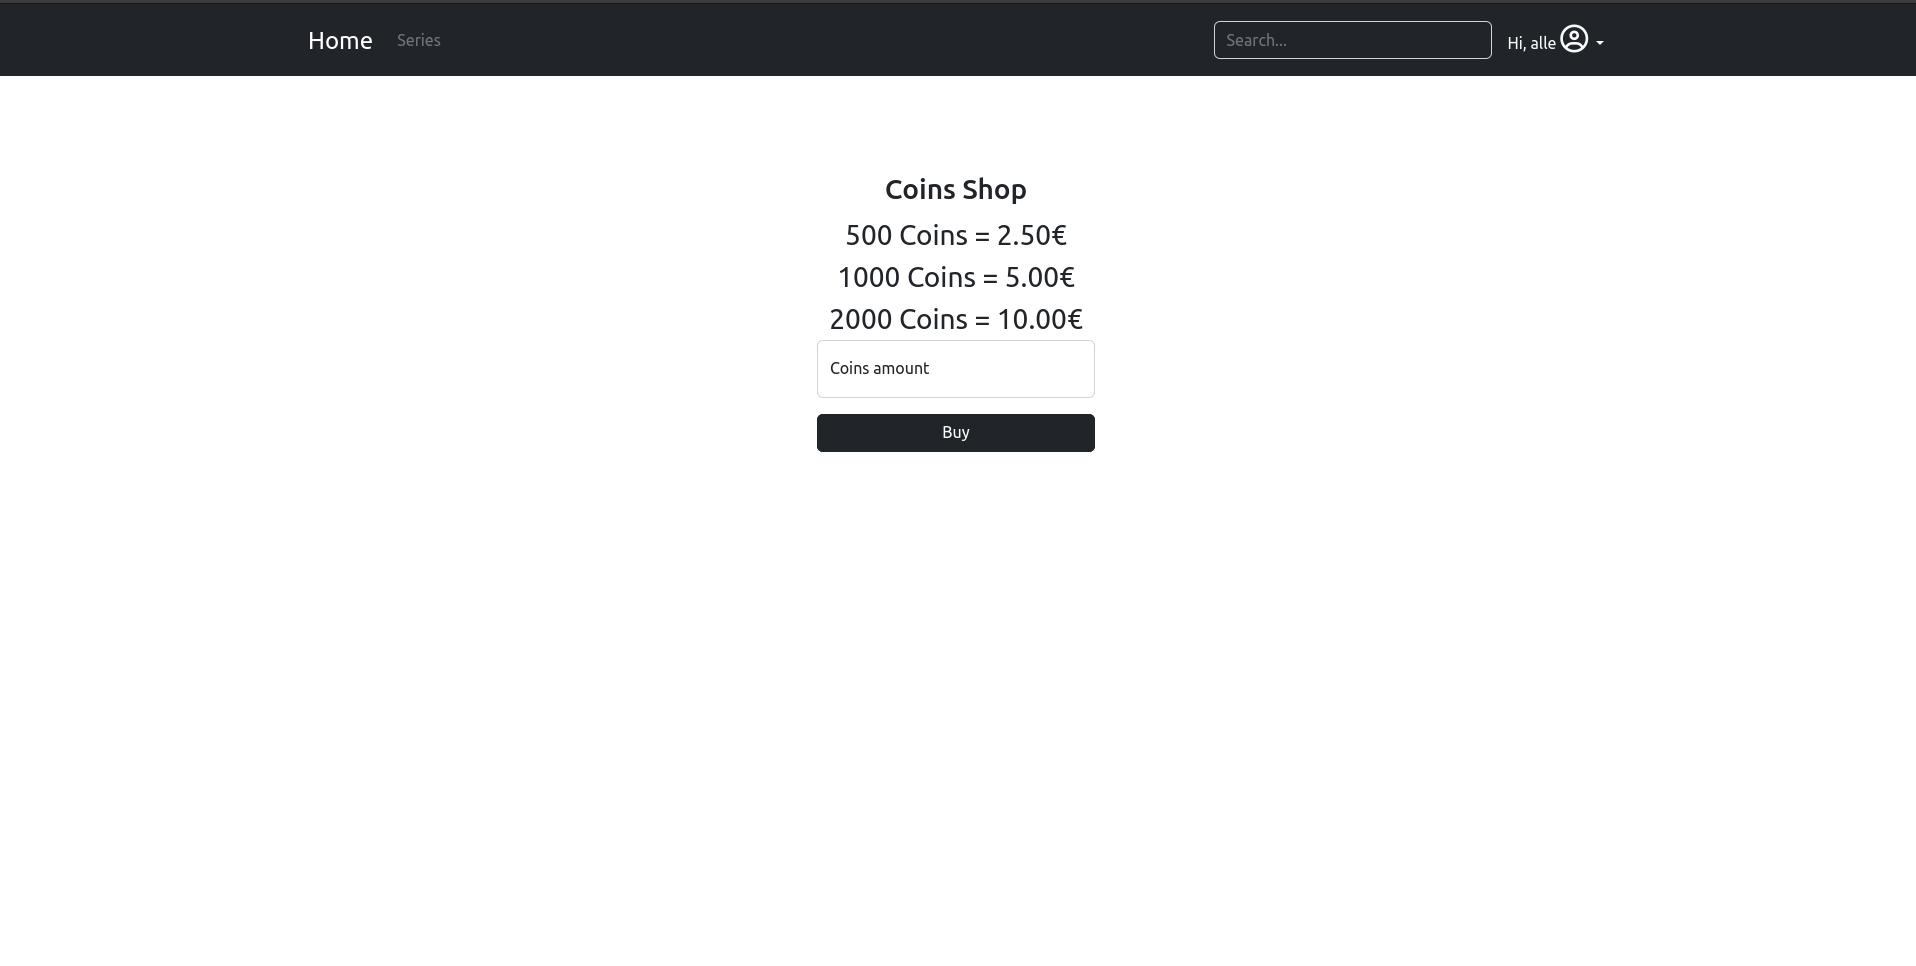
\includegraphics[width=1.0\linewidth]{images/market.png}

\subsection{My comics}
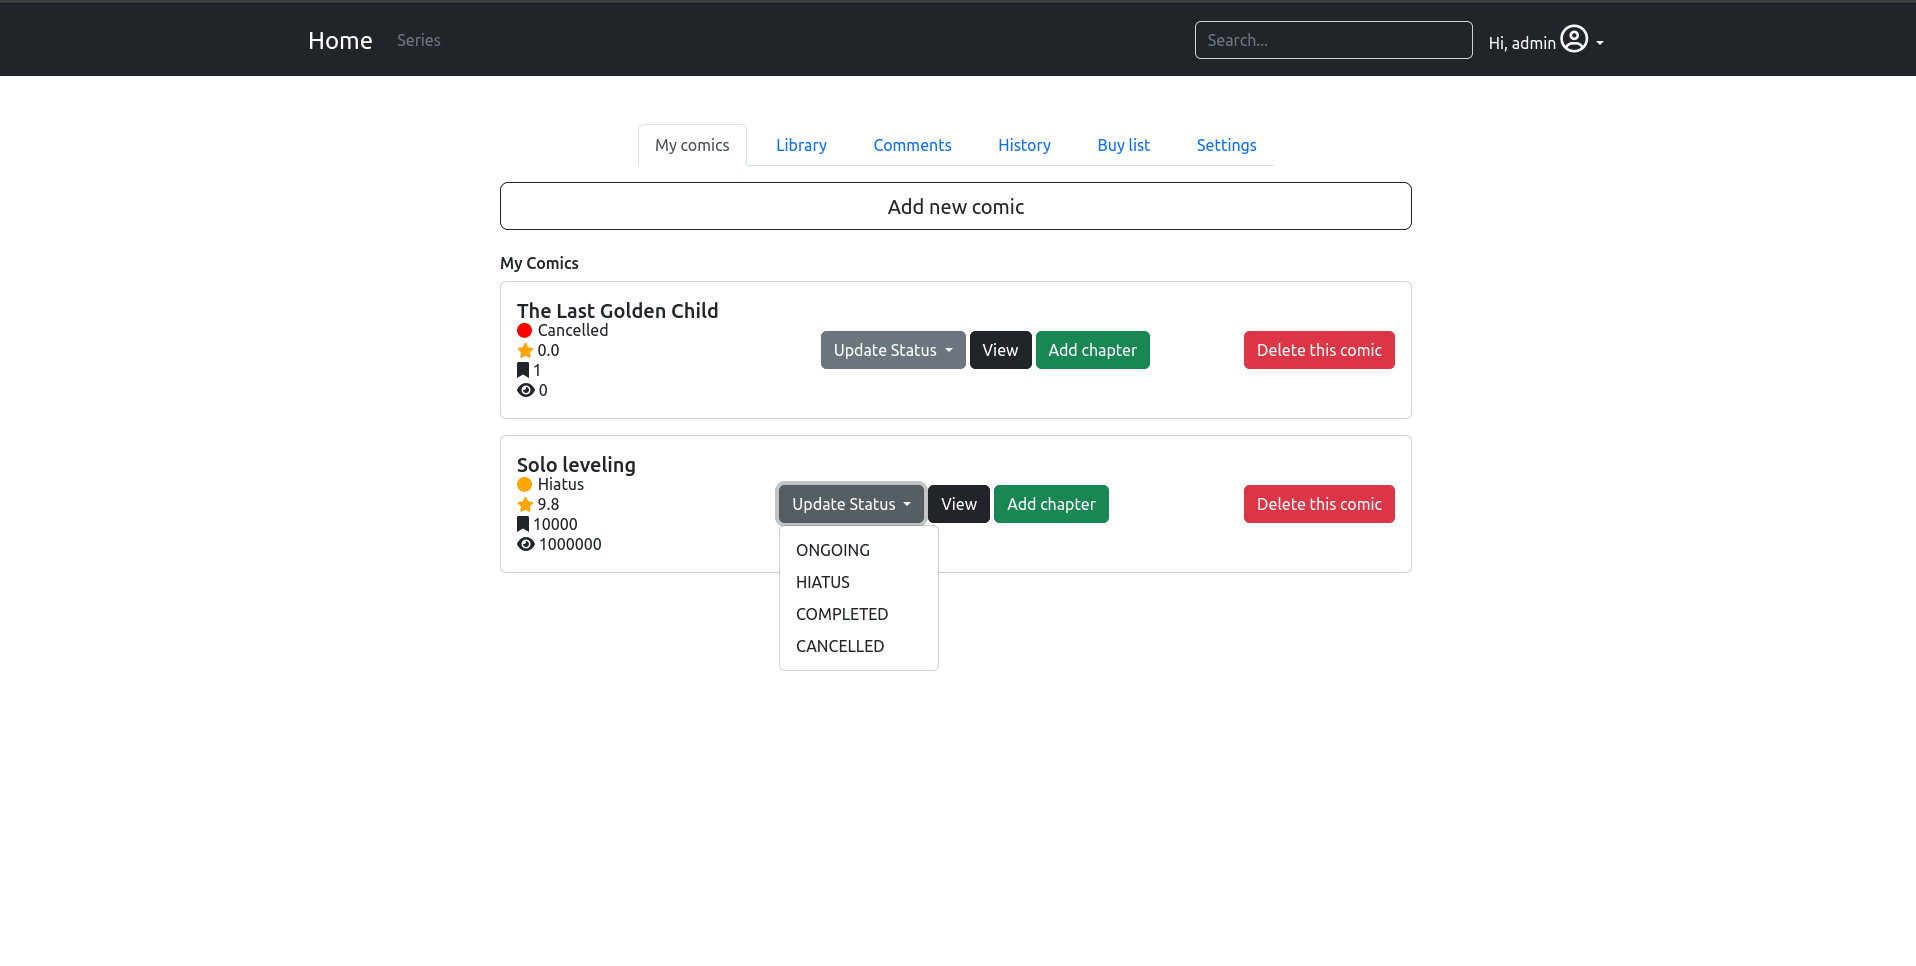
\includegraphics[width=1.0\linewidth]{images/my-comics.png}

\subsection{Add comic}
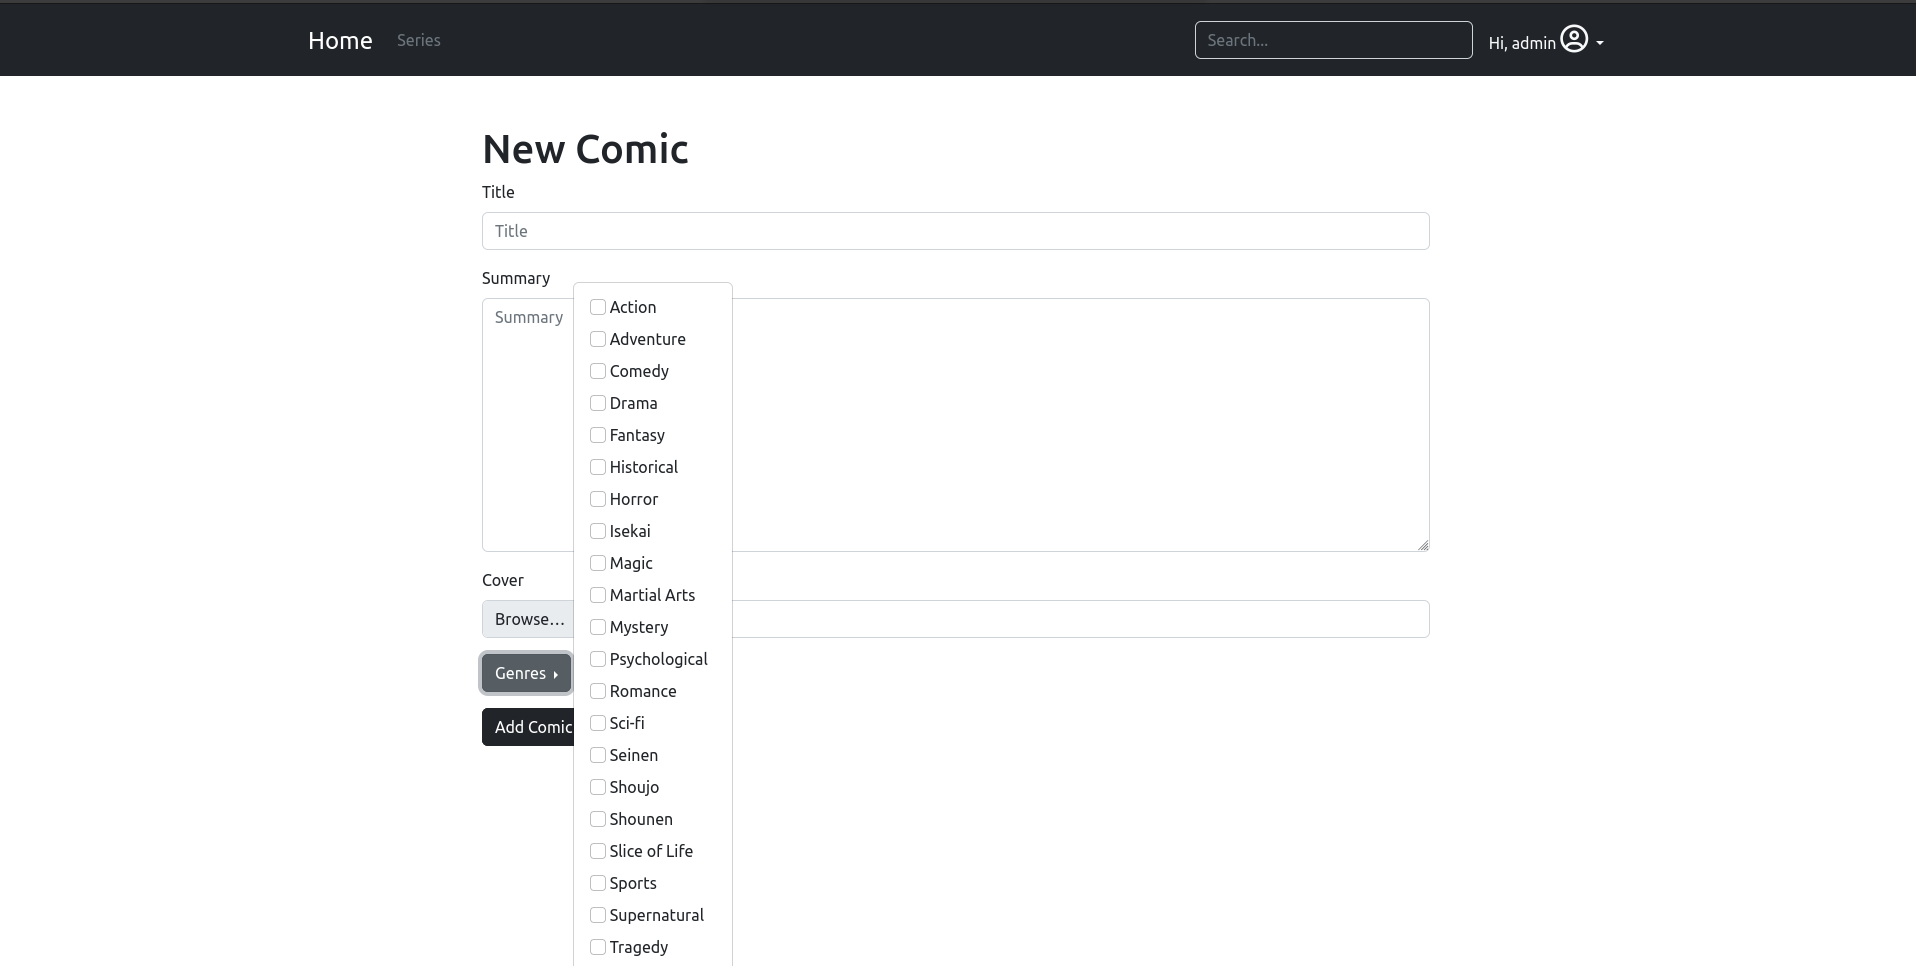
\includegraphics[width=1.0\linewidth]{images/new-comic.png}

\subsection{Add chapter}
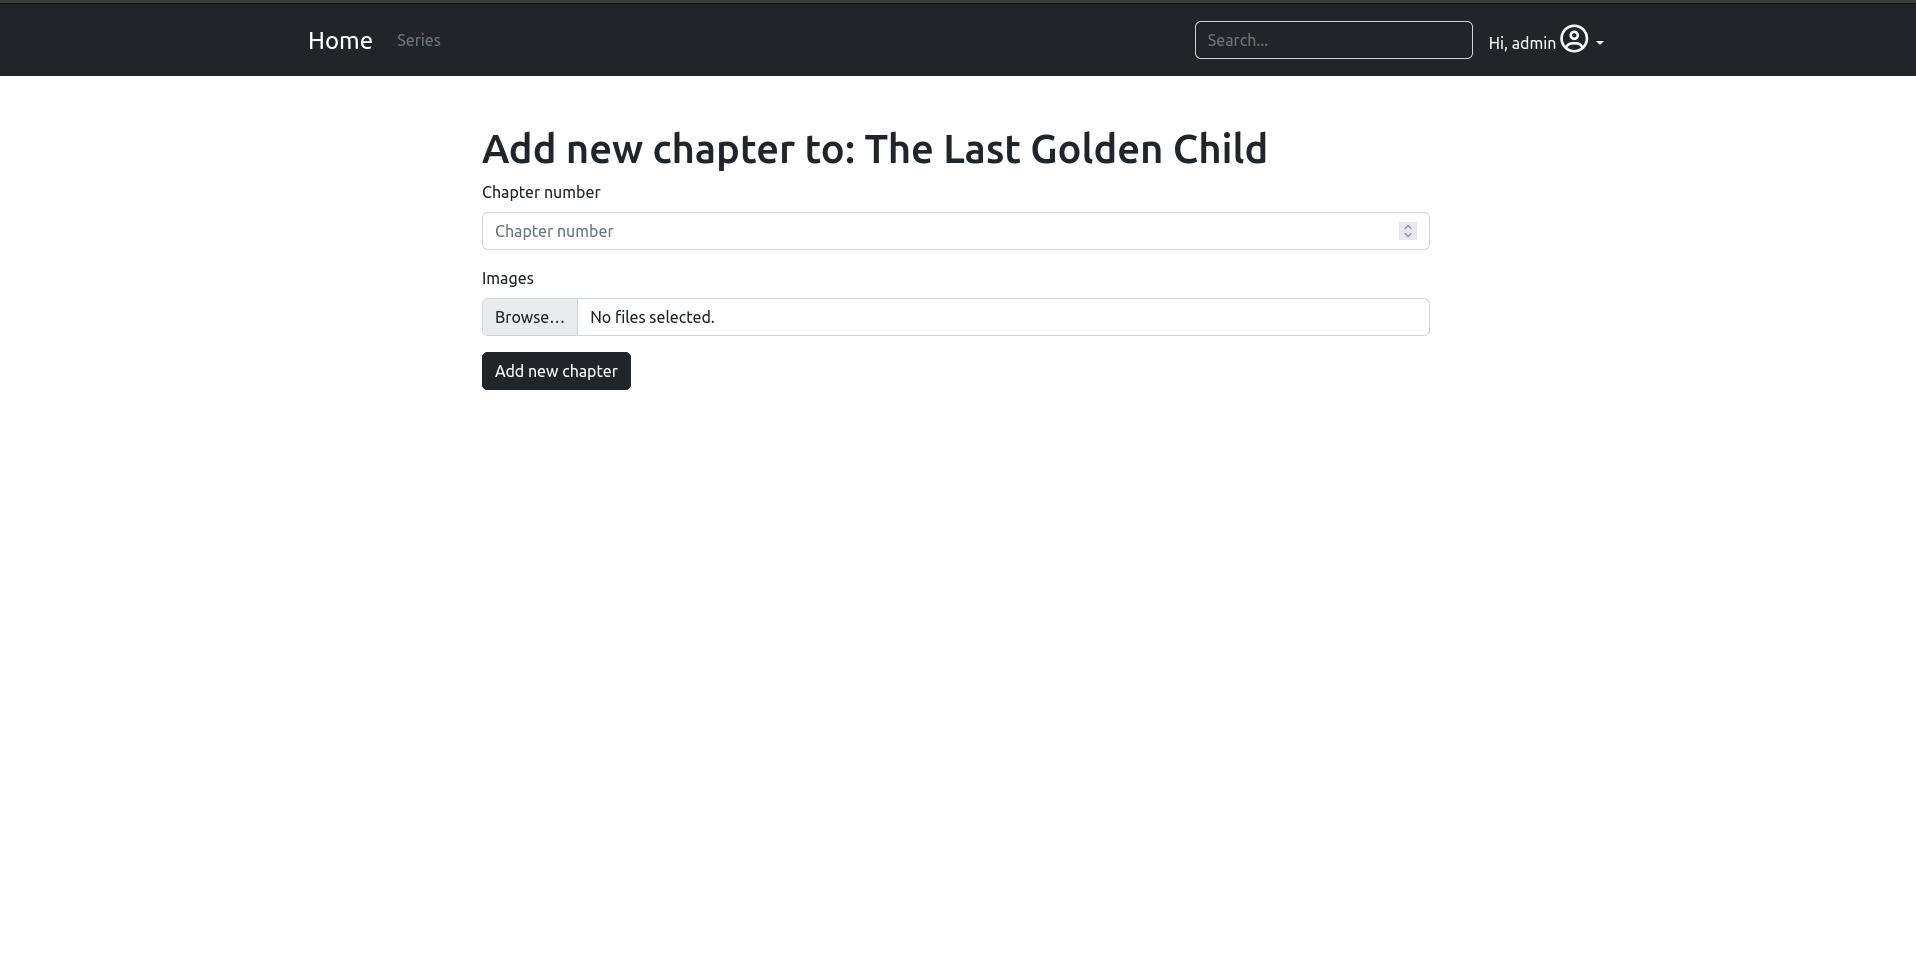
\includegraphics[width=1.0\linewidth]{images/new-chapter.png}


\break
\section{Problemi riscontrati}
Oltre alla familiarizzazione con Django, i problemi riscontrati sono stati pochi.
Oltre al problema del salvataggio delle immagini, risolto con un pacchetto di python,
l'unico altro problema riscontrato è stato passare il token CSRF (cross-site request forgery) in modo corretto tramite AJAX.
Fortunatamente sono state trovate soluzioni su internet, grazie ad altre persone che avevano già riscontrato questo problema.

\end{document}